\documentclass[1p]{elsarticle_modified}
%\bibliographystyle{elsarticle-num}

%\usepackage[colorlinks]{hyperref}
%\usepackage{abbrmath_seonhwa} %\Abb, \Ascr, \Acal ,\Abf, \Afrak
\usepackage{amsfonts}
\usepackage{amssymb}
\usepackage{amsmath}
\usepackage{amsthm}
\usepackage{scalefnt}
\usepackage{amsbsy}
\usepackage{kotex}
\usepackage{caption}
\usepackage{subfig}
\usepackage{color}
\usepackage{graphicx}
\usepackage{xcolor} %% white, black, red, green, blue, cyan, magenta, yellow
\usepackage{float}
\usepackage{setspace}
\usepackage{hyperref}

\usepackage{tikz}
\usetikzlibrary{arrows}

\usepackage{multirow}
\usepackage{array} % fixed length table
\usepackage{hhline}

%%%%%%%%%%%%%%%%%%%%%
\makeatletter
\renewcommand*\env@matrix[1][\arraystretch]{%
	\edef\arraystretch{#1}%
	\hskip -\arraycolsep
	\let\@ifnextchar\new@ifnextchar
	\array{*\c@MaxMatrixCols c}}
\makeatother %https://tex.stackexchange.com/questions/14071/how-can-i-increase-the-line-spacing-in-a-matrix
%%%%%%%%%%%%%%%

\usepackage[normalem]{ulem}

\newcommand{\msout}[1]{\ifmmode\text{\sout{\ensuremath{#1}}}\else\sout{#1}\fi}
%SOURCE: \msout is \stkout macro in https://tex.stackexchange.com/questions/20609/strikeout-in-math-mode

\newcommand{\cancel}[1]{
	\ifmmode
	{\color{red}\msout{#1}}
	\else
	{\color{red}\sout{#1}}
	\fi
}

\newcommand{\add}[1]{
	{\color{blue}\uwave{#1}}
}

\newcommand{\replace}[2]{
	\ifmmode
	{\color{red}\msout{#1}}{\color{blue}\uwave{#2}}
	\else
	{\color{red}\sout{#1}}{\color{blue}\uwave{#2}}
	\fi
}

\newcommand{\Sol}{\mathcal{S}} %segment
\newcommand{\D}{D} %diagram
\newcommand{\A}{\mathcal{A}} %arc


%%%%%%%%%%%%%%%%%%%%%%%%%%%%%5 test

\def\sl{\operatorname{\textup{SL}}(2,\Cbb)}
\def\psl{\operatorname{\textup{PSL}}(2,\Cbb)}
\def\quan{\mkern 1mu \triangleright \mkern 1mu}

\theoremstyle{definition}
\newtheorem{thm}{Theorem}[section]
\newtheorem{prop}[thm]{Proposition}
\newtheorem{lem}[thm]{Lemma}
\newtheorem{ques}[thm]{Question}
\newtheorem{cor}[thm]{Corollary}
\newtheorem{defn}[thm]{Definition}
\newtheorem{exam}[thm]{Example}
\newtheorem{rmk}[thm]{Remark}
\newtheorem{alg}[thm]{Algorithm}

\newcommand{\I}{\sqrt{-1}}
\begin{document}

%\begin{frontmatter}
%
%\title{Boundary parabolic representations of knots up to 8 crossings}
%
%%% Group authors per affiliation:
%\author{Yunhi Cho} 
%\address{Department of Mathematics, University of Seoul, Seoul, Korea}
%\ead{yhcho@uos.ac.kr}
%
%
%\author{Seonhwa Kim} %\fnref{s_kim}}
%\address{Center for Geometry and Physics, Institute for Basic Science, Pohang, 37673, Korea}
%\ead{ryeona17@ibs.re.kr}
%
%\author{Hyuk Kim}
%\address{Department of Mathematical Sciences, Seoul National University, Seoul 08826, Korea}
%\ead{hyukkim@snu.ac.kr}
%
%\author{Seokbeom Yoon}
%\address{Department of Mathematical Sciences, Seoul National University, Seoul, 08826,  Korea}
%\ead{sbyoon15@snu.ac.kr}
%
%\begin{abstract}
%We find all boundary parabolic representation of knots up to 8 crossings.
%
%\end{abstract}
%\begin{keyword}
%    \MSC[2010] 57M25 
%\end{keyword}
%
%\end{frontmatter}

%\linenumbers
%\tableofcontents
%
\newcommand\colored[1]{\textcolor{white}{\rule[-0.35ex]{0.8em}{1.4ex}}\kern-0.8em\color{red} #1}%
%\newcommand\colored[1]{\textcolor{white}{ #1}\kern-2.17ex	\textcolor{white}{ #1}\kern-1.81ex	\textcolor{white}{ #1}\kern-2.15ex\color{red}#1	}

{\Large $\underline{12a_{0785}~(K12a_{0785})}$}

\setlength{\tabcolsep}{10pt}
\renewcommand{\arraystretch}{1.6}
\vspace{1cm}\begin{tabular}{m{100pt}>{\centering\arraybackslash}m{274pt}}
\multirow{5}{120pt}{
	\centering
	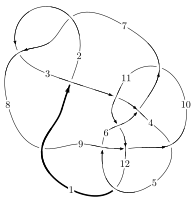
\includegraphics[width=112pt]{../../../GIT/diagram.site/Diagrams/png/1586_12a_0785.png}\\
\ \ \ A knot diagram\footnotemark}&
\allowdisplaybreaks
\textbf{Linearized knot diagam} \\
\cline{2-2}
 &
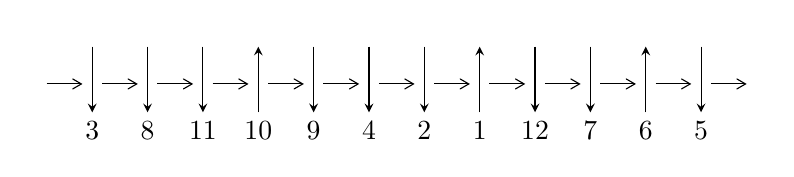
\begin{tikzpicture}[x=20pt, y=17pt]
	% nodes
	\node (C0) at (0, 0) {};
	\node (C1) at (1, 0) {};
	\node (C1U) at (1, +1) {};
	\node (C1D) at (1, -1) {3};

	\node (C2) at (2, 0) {};
	\node (C2U) at (2, +1) {};
	\node (C2D) at (2, -1) {8};

	\node (C3) at (3, 0) {};
	\node (C3U) at (3, +1) {};
	\node (C3D) at (3, -1) {11};

	\node (C4) at (4, 0) {};
	\node (C4U) at (4, +1) {};
	\node (C4D) at (4, -1) {10};

	\node (C5) at (5, 0) {};
	\node (C5U) at (5, +1) {};
	\node (C5D) at (5, -1) {9};

	\node (C6) at (6, 0) {};
	\node (C6U) at (6, +1) {};
	\node (C6D) at (6, -1) {4};

	\node (C7) at (7, 0) {};
	\node (C7U) at (7, +1) {};
	\node (C7D) at (7, -1) {2};

	\node (C8) at (8, 0) {};
	\node (C8U) at (8, +1) {};
	\node (C8D) at (8, -1) {1};

	\node (C9) at (9, 0) {};
	\node (C9U) at (9, +1) {};
	\node (C9D) at (9, -1) {12};

	\node (C10) at (10, 0) {};
	\node (C10U) at (10, +1) {};
	\node (C10D) at (10, -1) {7};

	\node (C11) at (11, 0) {};
	\node (C11U) at (11, +1) {};
	\node (C11D) at (11, -1) {6};

	\node (C12) at (12, 0) {};
	\node (C12U) at (12, +1) {};
	\node (C12D) at (12, -1) {5};
	\node (C13) at (13, 0) {};

	% arrows
	\draw[->,>={angle 60}]
	(C0) edge (C1) (C1) edge (C2) (C2) edge (C3) (C3) edge (C4) (C4) edge (C5) (C5) edge (C6) (C6) edge (C7) (C7) edge (C8) (C8) edge (C9) (C9) edge (C10) (C10) edge (C11) (C11) edge (C12) (C12) edge (C13) ;	\draw[->,>=stealth]
	(C1U) edge (C1D) (C2U) edge (C2D) (C3U) edge (C3D) (C4D) edge (C4U) (C5U) edge (C5D) (C6U) edge (C6D) (C7U) edge (C7D) (C8D) edge (C8U) (C9U) edge (C9D) (C10U) edge (C10D) (C11D) edge (C11U) (C12U) edge (C12D) ;
	\end{tikzpicture} \\
\hhline{~~} \\& 
\textbf{Solving Sequence} \\ \cline{2-2} 
 &
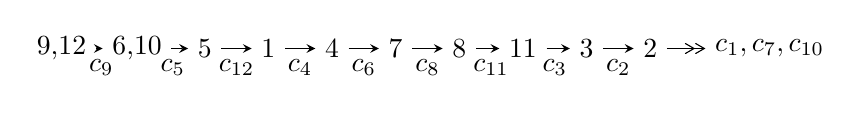
\begin{tikzpicture}[x=23pt, y=7pt]
	% node
	\node (A0) at (-1/8, 0) {9,12};
	\node (A1) at (17/16, 0) {6,10};
	\node (A2) at (17/8, 0) {5};
	\node (A3) at (25/8, 0) {1};
	\node (A4) at (33/8, 0) {4};
	\node (A5) at (41/8, 0) {7};
	\node (A6) at (49/8, 0) {8};
	\node (A7) at (57/8, 0) {11};
	\node (A8) at (65/8, 0) {3};
	\node (A9) at (73/8, 0) {2};
	\node (C1) at (1/2, -1) {$c_{9}$};
	\node (C2) at (13/8, -1) {$c_{5}$};
	\node (C3) at (21/8, -1) {$c_{12}$};
	\node (C4) at (29/8, -1) {$c_{4}$};
	\node (C5) at (37/8, -1) {$c_{6}$};
	\node (C6) at (45/8, -1) {$c_{8}$};
	\node (C7) at (53/8, -1) {$c_{11}$};
	\node (C8) at (61/8, -1) {$c_{3}$};
	\node (C9) at (69/8, -1) {$c_{2}$};
	\node (A10) at (11, 0) {$c_{1},c_{7},c_{10}$};

	% edge
	\draw[->,>=stealth]	
	(A0) edge (A1) (A1) edge (A2) (A2) edge (A3) (A3) edge (A4) (A4) edge (A5) (A5) edge (A6) (A6) edge (A7) (A7) edge (A8) (A8) edge (A9) ;
	\draw[->>,>={angle 60}]	
	(A9) edge (A10);
\end{tikzpicture} \\ 

\end{tabular} \\

\footnotetext{
The image of knot diagram is generated by the software ``\textbf{Draw programme}" developed by Andrew Bartholomew(\url{http://www.layer8.co.uk/maths/draw/index.htm\#Running-draw}), where we modified some parts for our purpose(\url{https://github.com/CATsTAILs/LinksPainter}).
}\phantom \\ \newline 
\centering \textbf{Ideals for irreducible components\footnotemark of $X_{\text{par}}$} 
 
\begin{align*}
I^u_{1}&=\langle 
-440 u^{19}-7822 u^{18}+\cdots+b-83010,\;101350 u^{19}+1884588 u^{18}+\cdots+419 a+33060194,\\
\phantom{I^u_{1}}&\phantom{= \langle  }u^{20}+19 u^{19}+\cdots+4045 u+419\rangle \\
I^u_{2}&=\langle 
-55 u^{25}-1474 u^{24}+\cdots+b-140189,\;-17044 u^{25}-361672 u^{24}+\cdots+2239 a+75396086,\\
\phantom{I^u_{2}}&\phantom{= \langle  }u^{26}+27 u^{25}+\cdots+29107 u+2239\rangle \\
I^u_{3}&=\langle 
-5.90378\times10^{27} a^{17} u^{3}+2.02102\times10^{27} a^{16} u^{3}+\cdots-6.93993\times10^{27} a-7.66958\times10^{27},\\
\phantom{I^u_{3}}&\phantom{= \langle  }- a^{17} u^3-3 a^{16} u^3+\cdots-143936 a+299131,\;u^4- u^3+2 u+1\rangle \\
I^u_{4}&=\langle 
8.04582\times10^{32} a^{17} u+5.01372\times10^{32} a^{16} u+\cdots-7.33139\times10^{32} a-5.03241\times10^{33},\\
\phantom{I^u_{4}}&\phantom{= \langle  }-2 a^{17} u+3 a^{16} u+\cdots+36 a+9,\;u^2- u+1\rangle \\
I^u_{5}&=\langle 
1.00210\times10^{26} u^{37}-1.30856\times10^{27} u^{36}+\cdots+8.88085\times10^{25} b-1.95986\times10^{26},\\
\phantom{I^u_{5}}&\phantom{= \langle  }9.57765\times10^{25} u^{37}-1.33504\times10^{27} u^{36}+\cdots+8.88085\times10^{25} a-6.26187\times10^{25},\;u^{38}-14 u^{37}+\cdots+u+1\rangle \\
I^u_{6}&=\langle 
b^2+b a- a^2-1,\;a^9- a^8+2 a^7- a^6+3 a^5- a^4+2 a^3+a+1,\;u-1\rangle \\
I^u_{7}&=\langle 
b+1,\;a,\;u-1\rangle \\
\\
I^v_{1}&=\langle 
a,\;b^9+b^8+2 b^7+b^6+3 b^5+b^4+2 b^3+b-1,\;v-1\rangle \\
\end{align*}
\raggedright * 8 irreducible components of $\dim_{\mathbb{C}}=0$, with total 220 representations.\\
\footnotetext{All coefficients of polynomials are rational numbers. But the coefficients are sometimes approximated in decimal forms when there is not enough margin.}
\newpage
\renewcommand{\arraystretch}{1}
\centering \section*{I. $I^u_{1}= \langle -440 u^{19}-7822 u^{18}+\cdots+b-83010,\;1.01\times10^{5} u^{19}+1.88\times10^{6} u^{18}+\cdots+419 a+3.31\times10^{7},\;u^{20}+19 u^{19}+\cdots+4045 u+419 \rangle$}
\flushleft \textbf{(i) Arc colorings}\\
\begin{tabular}{m{7pt} m{180pt} m{7pt} m{180pt} }
\flushright $a_{9}=$&$\begin{pmatrix}1\\0\end{pmatrix}$ \\
\flushright $a_{12}=$&$\begin{pmatrix}0\\u\end{pmatrix}$ \\
\flushright $a_{6}=$&$\begin{pmatrix}-241.885 u^{19}-4497.82 u^{18}+\cdots-728143. u-78902.6\\440 u^{19}+7822 u^{18}+\cdots+797266 u+83010\end{pmatrix}$ \\
\flushright $a_{10}=$&$\begin{pmatrix}1\\u^2\end{pmatrix}$ \\
\flushright $a_{5}=$&$\begin{pmatrix}198.115 u^{19}+3324.18 u^{18}+\cdots+69123.0 u+4107.39\\440 u^{19}+7822 u^{18}+\cdots+797266 u+83010\end{pmatrix}$ \\
\flushright $a_{1}=$&$\begin{pmatrix}0.498807 u^{19}+8.47733 u^{18}+\cdots+82.9165 u-5.32697\\u^{19}+18 u^{18}+\cdots+2024 u+209\end{pmatrix}$ \\
\flushright $a_{4}=$&$\begin{pmatrix}296.115 u^{19}+5559.18 u^{18}+\cdots+968647. u+105457.\\-679 u^{19}-11745 u^{18}+\cdots-752581 u-73277\end{pmatrix}$ \\
\flushright $a_{7}=$&$\begin{pmatrix}-174.885 u^{19}-2643.82 u^{18}+\cdots+364183. u+45169.4\\-716 u^{19}-13126 u^{18}+\cdots-1876012 u-201491\end{pmatrix}$ \\
\flushright $a_{8}=$&$\begin{pmatrix}4.25060 u^{19}+81.7613 u^{18}+\cdots+18071.5 u+1994.66\\-2 u^{19}-27 u^{18}+\cdots+11364 u+1362\end{pmatrix}$ \\
\flushright $a_{11}=$&$\begin{pmatrix}-0.501193 u^{19}-8.52267 u^{18}+\cdots-127.084 u-4.32697\\- u^{18}-17 u^{17}+\cdots-1812 u-210\end{pmatrix}$ \\
\flushright $a_{3}=$&$\begin{pmatrix}-532.943 u^{19}-9436.91 u^{18}+\cdots-915041. u-94759.3\\-73 u^{19}-1966 u^{18}+\cdots-1107172 u-125676\end{pmatrix}$ \\
\flushright $a_{2}=$&$\begin{pmatrix}10.5609 u^{19}+95.6563 u^{18}+\cdots-125604. u-14672.3\\90 u^{19}+1670 u^{18}+\cdots+266050 u+28727\end{pmatrix}$\\&\end{tabular}
\flushleft \textbf{(ii) Obstruction class $= -1$}\\~\\
\flushleft \textbf{(iii) Cusp Shapes $= -272 u^{19}-4238 u^{18}-31694 u^{17}-149912 u^{16}-499032 u^{15}-1231956 u^{14}-2311268 u^{13}-3295698 u^{12}-3426358 u^{11}-2150740 u^{10}+263316 u^9+2695132 u^8+4037400 u^7+4211956 u^6+3957808 u^5+3582696 u^4+2698114 u^3+1385042 u^2+391594 u+50234$}\\~\\
\newpage\renewcommand{\arraystretch}{1}
\flushleft \textbf{(iv) u-Polynomials at the component}\newline \\
\begin{tabular}{m{50pt}|m{274pt}}
Crossings & \hspace{64pt}u-Polynomials at each crossing \\
\hline $$\begin{aligned}c_{1}\end{aligned}$$&$\begin{aligned}
&u^{20}+10 u^{19}+\cdots-160 u+64
\end{aligned}$\\
\hline $$\begin{aligned}c_{2},c_{7}\end{aligned}$$&$\begin{aligned}
&u^{20}-6 u^{19}+\cdots-40 u+8
\end{aligned}$\\
\hline $$\begin{aligned}c_{3},c_{5},c_{10}\\c_{12}\end{aligned}$$&$\begin{aligned}
&u^{20}+u^{19}+\cdots- u+1
\end{aligned}$\\
\hline $$\begin{aligned}c_{4},c_{11}\end{aligned}$$&$\begin{aligned}
&u^{20}+u^{19}+\cdots+2 u+26
\end{aligned}$\\
\hline $$\begin{aligned}c_{6},c_{9}\end{aligned}$$&$\begin{aligned}
&u^{20}-19 u^{19}+\cdots-4045 u+419
\end{aligned}$\\
\hline $$\begin{aligned}c_{8}\end{aligned}$$&$\begin{aligned}
&u^{20}-18 u^{19}+\cdots-24920 u+3688
\end{aligned}$\\
\hline
\end{tabular}\\~\\
\newpage\renewcommand{\arraystretch}{1}
\flushleft \textbf{(v) Riley Polynomials at the component}\newline \\
\begin{tabular}{m{50pt}|m{274pt}}
Crossings & \hspace{64pt}Riley Polynomials at each crossing \\
\hline $$\begin{aligned}c_{1}\end{aligned}$$&$\begin{aligned}
&y^{20}-2 y^{19}+\cdots-23040 y+4096
\end{aligned}$\\
\hline $$\begin{aligned}c_{2},c_{7}\end{aligned}$$&$\begin{aligned}
&y^{20}-10 y^{19}+\cdots+160 y+64
\end{aligned}$\\
\hline $$\begin{aligned}c_{3},c_{5},c_{10}\\c_{12}\end{aligned}$$&$\begin{aligned}
&y^{20}- y^{19}+\cdots+11 y+1
\end{aligned}$\\
\hline $$\begin{aligned}c_{4},c_{11}\end{aligned}$$&$\begin{aligned}
&y^{20}+21 y^{19}+\cdots+10448 y+676
\end{aligned}$\\
\hline $$\begin{aligned}c_{6},c_{9}\end{aligned}$$&$\begin{aligned}
&y^{20}-9 y^{19}+\cdots-853997 y+175561
\end{aligned}$\\
\hline $$\begin{aligned}c_{8}\end{aligned}$$&$\begin{aligned}
&y^{20}-4 y^{19}+\cdots+14317984 y+13601344
\end{aligned}$\\
\hline
\end{tabular}\\~\\
\newpage\flushleft \textbf{(vi) Complex Volumes and Cusp Shapes}
$$\begin{array}{c|c|c}  
\text{Solutions to }I^u_{1}& \I (\text{vol} + \sqrt{-1}CS) & \text{Cusp shape}\\
 \hline 
\begin{aligned}
u &= \phantom{-}0.512099 + 0.698028 I \\
a &= -0.757073 - 0.694555 I \\
b &= \phantom{-}0.169556 + 0.506438 I\end{aligned}
 & -0.63165 - 1.63991 I & -3.29731 + 4.07135 I \\ \hline\begin{aligned}
u &= \phantom{-}0.512099 - 0.698028 I \\
a &= -0.757073 + 0.694555 I \\
b &= \phantom{-}0.169556 - 0.506438 I\end{aligned}
 & -0.63165 + 1.63991 I & -3.29731 - 4.07135 I \\ \hline\begin{aligned}
u &= \phantom{-}0.00580 + 1.43849 I \\
a &= \phantom{-}0.706982 + 0.120837 I \\
b &= -0.419757 - 0.411483 I\end{aligned}
 & -4.80670 - 5.98648 I & -6.00000 + 11.08698 I \\ \hline\begin{aligned}
u &= \phantom{-}0.00580 - 1.43849 I \\
a &= \phantom{-}0.706982 - 0.120837 I \\
b &= -0.419757 + 0.411483 I\end{aligned}
 & -4.80670 + 5.98648 I & -6.00000 - 11.08698 I \\ \hline\begin{aligned}
u &= -1.16335 + 1.05046 I \\
a &= -0.242193 + 1.117750 I \\
b &= \phantom{-}1.31614 - 1.05420 I\end{aligned}
 & -8.2024 + 21.0457 I & \phantom{-0.000000 } 0 \\ \hline\begin{aligned}
u &= -1.16335 - 1.05046 I \\
a &= -0.242193 - 1.117750 I \\
b &= \phantom{-}1.31614 + 1.05420 I\end{aligned}
 & -8.2024 - 21.0457 I & \phantom{-0.000000 } 0 \\ \hline\begin{aligned}
u &= -1.17748 + 1.05342 I \\
a &= \phantom{-}0.232775 - 1.068910 I \\
b &= -1.25568 + 1.02028 I\end{aligned}
 & -5.1187 + 15.7823 I & \phantom{-0.000000 } 0 \\ \hline\begin{aligned}
u &= -1.17748 - 1.05342 I \\
a &= \phantom{-}0.232775 + 1.068910 I \\
b &= -1.25568 - 1.02028 I\end{aligned}
 & -5.1187 - 15.7823 I & \phantom{-0.000000 } 0 \\ \hline\begin{aligned}
u &= -1.17927 + 1.07828 I \\
a &= -0.298894 + 1.028330 I \\
b &= \phantom{-}1.27177 - 0.91287 I\end{aligned}
 & -9.8158 + 11.6670 I & \phantom{-0.000000 } 0 \\ \hline\begin{aligned}
u &= -1.17927 - 1.07828 I \\
a &= -0.298894 - 1.028330 I \\
b &= \phantom{-}1.27177 + 0.91287 I\end{aligned}
 & -9.8158 - 11.6670 I & \phantom{-0.000000 } 0\\
 \hline 
 \end{array}$$\newpage$$\begin{array}{c|c|c}  
\text{Solutions to }I^u_{1}& \I (\text{vol} + \sqrt{-1}CS) & \text{Cusp shape}\\
 \hline 
\begin{aligned}
u &= -1.26927 + 1.01007 I \\
a &= \phantom{-}0.086517 - 0.867442 I \\
b &= -0.909643 + 1.001230 I\end{aligned}
 & -0.48741 + 13.75390 I & \phantom{-0.000000 } 0 \\ \hline\begin{aligned}
u &= -1.26927 - 1.01007 I \\
a &= \phantom{-}0.086517 + 0.867442 I \\
b &= -0.909643 - 1.001230 I\end{aligned}
 & -0.48741 - 13.75390 I & \phantom{-0.000000 } 0 \\ \hline\begin{aligned}
u &= -0.290662 + 0.201866 I \\
a &= -1.20981 + 1.20451 I \\
b &= \phantom{-}0.079084 + 0.815354 I\end{aligned}
 & \phantom{-}1.78290 - 2.14893 I & \phantom{-}0.04329 + 4.23950 I \\ \hline\begin{aligned}
u &= -0.290662 - 0.201866 I \\
a &= -1.20981 - 1.20451 I \\
b &= \phantom{-}0.079084 - 0.815354 I\end{aligned}
 & \phantom{-}1.78290 + 2.14893 I & \phantom{-}0.04329 - 4.23950 I \\ \hline\begin{aligned}
u &= -1.34983 + 0.99384 I \\
a &= -0.068669 + 0.743707 I \\
b &= \phantom{-}0.756125 - 0.916597 I\end{aligned}
 & \phantom{-}0.45556 + 8.22051 I & \phantom{-0.000000 } 0 \\ \hline\begin{aligned}
u &= -1.34983 - 0.99384 I \\
a &= -0.068669 - 0.743707 I \\
b &= \phantom{-}0.756125 + 0.916597 I\end{aligned}
 & \phantom{-}0.45556 - 8.22051 I & \phantom{-0.000000 } 0 \\ \hline\begin{aligned}
u &= -1.49300 + 1.31522 I \\
a &= \phantom{-}0.274286 - 0.533423 I \\
b &= -0.698441 + 0.483867 I\end{aligned}
 & -7.23704 + 6.69767 I & \phantom{-0.000000 } 0 \\ \hline\begin{aligned}
u &= -1.49300 - 1.31522 I \\
a &= \phantom{-}0.274286 + 0.533423 I \\
b &= -0.698441 - 0.483867 I\end{aligned}
 & -7.23704 - 6.69767 I & \phantom{-0.000000 } 0 \\ \hline\begin{aligned}
u &= -2.09503 + 0.56369 I \\
a &= -0.029412 + 0.377289 I \\
b &= \phantom{-}0.190855 - 0.638731 I\end{aligned}
 & \phantom{-}0.34008 + 3.38661 I & \phantom{-0.000000 } 0 \\ \hline\begin{aligned}
u &= -2.09503 - 0.56369 I \\
a &= -0.029412 - 0.377289 I \\
b &= \phantom{-}0.190855 + 0.638731 I\end{aligned}
 & \phantom{-}0.34008 - 3.38661 I & \phantom{-0.000000 } 0\\
 \hline 
 \end{array}$$\newpage\newpage\renewcommand{\arraystretch}{1}
\centering \section*{II. $I^u_{2}= \langle -55 u^{25}-1474 u^{24}+\cdots+b-140189,\;-1.70\times10^{4} u^{25}-3.62\times10^{5} u^{24}+\cdots+2239 a+7.54\times10^{7},\;u^{26}+27 u^{25}+\cdots+29107 u+2239 \rangle$}
\flushleft \textbf{(i) Arc colorings}\\
\begin{tabular}{m{7pt} m{180pt} m{7pt} m{180pt} }
\flushright $a_{9}=$&$\begin{pmatrix}1\\0\end{pmatrix}$ \\
\flushright $a_{12}=$&$\begin{pmatrix}0\\u\end{pmatrix}$ \\
\flushright $a_{6}=$&$\begin{pmatrix}7.61233 u^{25}+161.533 u^{24}+\cdots-386377. u-33674\\55 u^{25}+1474 u^{24}+\cdots+1715942 u+140189\end{pmatrix}$ \\
\flushright $a_{10}=$&$\begin{pmatrix}1\\u^2\end{pmatrix}$ \\
\flushright $a_{5}=$&$\begin{pmatrix}62.6123 u^{25}+1635.53 u^{24}+\cdots+1.32957\times10^{6} u+106515\\55 u^{25}+1474 u^{24}+\cdots+1715942 u+140189\end{pmatrix}$ \\
\flushright $a_{1}=$&$\begin{pmatrix}-1.49978 u^{25}-39.4940 u^{24}+\cdots-40819.5 u-3351\\- u^{25}-27 u^{24}+\cdots-40302 u-3358\end{pmatrix}$ \\
\flushright $a_{4}=$&$\begin{pmatrix}18.6123 u^{25}+533.533 u^{24}+\cdots+1.07432\times10^{6} u+89471\\-62 u^{25}-1572 u^{24}+\cdots-688744 u-52365\end{pmatrix}$ \\
\flushright $a_{7}=$&$\begin{pmatrix}129.612 u^{25}+3364.53 u^{24}+\cdots+2.48091\times10^{6} u+197811\\29 u^{25}+900 u^{24}+\cdots+2630825 u+220793\end{pmatrix}$ \\
\flushright $a_{8}=$&$\begin{pmatrix}4.25011 u^{25}+105.753 u^{24}+\cdots-539.268 u-555\\9 u^{25}+233 u^{24}+\cdots+150013 u+11755\end{pmatrix}$ \\
\flushright $a_{11}=$&$\begin{pmatrix}0.500223 u^{25}+13.5060 u^{24}+\cdots+14037.5 u+1126\\- u^{25}-26 u^{24}+\cdots-14553 u-1119\end{pmatrix}$ \\
\flushright $a_{3}=$&$\begin{pmatrix}43.4185 u^{25}+1199.30 u^{24}+\cdots+1.88287\times10^{6} u+155911\\-113 u^{25}-2859 u^{24}+\cdots-1150846 u-86384\end{pmatrix}$ \\
\flushright $a_{2}=$&$\begin{pmatrix}-41.1867 u^{25}-1062.04 u^{24}+\cdots-628304. u-48954\\-3 u^{25}-119 u^{24}+\cdots-642593 u-54154\end{pmatrix}$\\&\end{tabular}
\flushleft \textbf{(ii) Obstruction class $= -1$}\\~\\
\flushleft \textbf{(iii) Cusp Shapes $= 115 u^{25}+2941 u^{24}+\cdots+1504608 u+115595$}\\~\\
\newpage\renewcommand{\arraystretch}{1}
\flushleft \textbf{(iv) u-Polynomials at the component}\newline \\
\begin{tabular}{m{50pt}|m{274pt}}
Crossings & \hspace{64pt}u-Polynomials at each crossing \\
\hline $$\begin{aligned}c_{1}\end{aligned}$$&$\begin{aligned}
&(u^{13}+6 u^{12}+\cdots+12 u+16)^{2}
\end{aligned}$\\
\hline $$\begin{aligned}c_{2},c_{7}\end{aligned}$$&$\begin{aligned}
&(u^{13}-4 u^{12}+\cdots-14 u+4)^{2}
\end{aligned}$\\
\hline $$\begin{aligned}c_{3},c_{5},c_{10}\\c_{12}\end{aligned}$$&$\begin{aligned}
&u^{26}+u^{25}+\cdots+u+1
\end{aligned}$\\
\hline $$\begin{aligned}c_{4},c_{11}\end{aligned}$$&$\begin{aligned}
&(u^{13}+u^{11}+u^{10}-2 u^7- u^6- u^5-2 u^4+u^3+u^2+u+1)^2
\end{aligned}$\\
\hline $$\begin{aligned}c_{6},c_{9}\end{aligned}$$&$\begin{aligned}
&u^{26}-27 u^{25}+\cdots-29107 u+2239
\end{aligned}$\\
\hline $$\begin{aligned}c_{8}\end{aligned}$$&$\begin{aligned}
&(u^{13}-12 u^{12}+\cdots+210 u+4)^{2}
\end{aligned}$\\
\hline
\end{tabular}\\~\\
\newpage\renewcommand{\arraystretch}{1}
\flushleft \textbf{(v) Riley Polynomials at the component}\newline \\
\begin{tabular}{m{50pt}|m{274pt}}
Crossings & \hspace{64pt}Riley Polynomials at each crossing \\
\hline $$\begin{aligned}c_{1}\end{aligned}$$&$\begin{aligned}
&(y^{13}+2 y^{12}+\cdots-656 y-256)^{2}
\end{aligned}$\\
\hline $$\begin{aligned}c_{2},c_{7}\end{aligned}$$&$\begin{aligned}
&(y^{13}-6 y^{12}+\cdots+12 y-16)^{2}
\end{aligned}$\\
\hline $$\begin{aligned}c_{3},c_{5},c_{10}\\c_{12}\end{aligned}$$&$\begin{aligned}
&y^{26}-3 y^{25}+\cdots- y+1
\end{aligned}$\\
\hline $$\begin{aligned}c_{4},c_{11}\end{aligned}$$&$\begin{aligned}
&(y^{13}+2 y^{12}+\cdots- y-1)^{2}
\end{aligned}$\\
\hline $$\begin{aligned}c_{6},c_{9}\end{aligned}$$&$\begin{aligned}
&y^{26}-13 y^{25}+\cdots+24344647 y+5013121
\end{aligned}$\\
\hline $$\begin{aligned}c_{8}\end{aligned}$$&$\begin{aligned}
&(y^{13}+2 y^{12}+\cdots+52908 y-16)^{2}
\end{aligned}$\\
\hline
\end{tabular}\\~\\
\newpage\flushleft \textbf{(vi) Complex Volumes and Cusp Shapes}
$$\begin{array}{c|c|c}  
\text{Solutions to }I^u_{2}& \I (\text{vol} + \sqrt{-1}CS) & \text{Cusp shape}\\
 \hline 
\begin{aligned}
u &= -0.666943 + 0.686087 I \\
a &= \phantom{-}0.512939 + 0.892142 I \\
b &= \phantom{-}0.833119 - 0.986335 I\end{aligned}
 & \phantom{-}2.19583 + 5.62038 I & \phantom{-0.000000 } 0 \\ \hline\begin{aligned}
u &= -0.666943 - 0.686087 I \\
a &= \phantom{-}0.512939 - 0.892142 I \\
b &= \phantom{-}0.833119 + 0.986335 I\end{aligned}
 & \phantom{-}2.19583 - 5.62038 I & \phantom{-0.000000 } 0 \\ \hline\begin{aligned}
u &= -0.570390 + 0.767585 I \\
a &= -0.523314 - 0.899263 I \\
b &= -0.659342 + 0.919109 I\end{aligned}
 & \phantom{-}3.66757 + 0.92622 I & \phantom{-0.000000 } 0 \\ \hline\begin{aligned}
u &= -0.570390 - 0.767585 I \\
a &= -0.523314 + 0.899263 I \\
b &= -0.659342 - 0.919109 I\end{aligned}
 & \phantom{-}3.66757 - 0.92622 I & \phantom{-0.000000 } 0 \\ \hline\begin{aligned}
u &= -0.444770 + 0.992031 I \\
a &= -0.465440 - 0.788020 I \\
b &= -0.339390 + 0.806743 I\end{aligned}
 & \phantom{-}3.66757 - 0.92622 I & \phantom{-0.000000 } 0 \\ \hline\begin{aligned}
u &= -0.444770 - 0.992031 I \\
a &= -0.465440 + 0.788020 I \\
b &= -0.339390 - 0.806743 I\end{aligned}
 & \phantom{-}3.66757 + 0.92622 I & \phantom{-0.000000 } 0 \\ \hline\begin{aligned}
u &= -0.427386 + 1.179570 I \\
a &= \phantom{-}0.441249 + 0.649055 I \\
b &= \phantom{-}0.151020 - 0.735618 I\end{aligned}
 & \phantom{-}2.19583 - 5.62038 I & \phantom{-0.000000 } 0 \\ \hline\begin{aligned}
u &= -0.427386 - 1.179570 I \\
a &= \phantom{-}0.441249 - 0.649055 I \\
b &= \phantom{-}0.151020 + 0.735618 I\end{aligned}
 & \phantom{-}2.19583 + 5.62038 I & \phantom{-0.000000 } 0 \\ \hline\begin{aligned}
u &= -1.132080 + 0.739477 I \\
a &= \phantom{-}0.070245 - 0.895176 I \\
b &= -1.25982 + 1.01265 I\end{aligned}
 & -7.7321 + 12.4192 I & \phantom{-0.000000 } 0 \\ \hline\begin{aligned}
u &= -1.132080 - 0.739477 I \\
a &= \phantom{-}0.070245 + 0.895176 I \\
b &= -1.25982 - 1.01265 I\end{aligned}
 & -7.7321 - 12.4192 I & \phantom{-0.000000 } 0\\
 \hline 
 \end{array}$$\newpage$$\begin{array}{c|c|c}  
\text{Solutions to }I^u_{2}& \I (\text{vol} + \sqrt{-1}CS) & \text{Cusp shape}\\
 \hline 
\begin{aligned}
u &= -1.164030 + 0.702554 I \\
a &= -0.062452 + 0.817215 I \\
b &= \phantom{-}1.18521 - 0.99046 I\end{aligned}
 & -4.61821 + 6.97339 I & \phantom{-0.000000 } 0 \\ \hline\begin{aligned}
u &= -1.164030 - 0.702554 I \\
a &= -0.062452 - 0.817215 I \\
b &= \phantom{-}1.18521 + 0.99046 I\end{aligned}
 & -4.61821 - 6.97339 I & \phantom{-0.000000 } 0 \\ \hline\begin{aligned}
u &= -0.184678 + 0.579008 I \\
a &= \phantom{-}0.391553 + 1.227610 I \\
b &= \phantom{-}0.638483 - 0.453424 I\end{aligned}
 & -0.986461\phantom{ +0.000000I} & -7.57792 + 0. I\phantom{ +0.000000I} \\ \hline\begin{aligned}
u &= -0.184678 - 0.579008 I \\
a &= \phantom{-}0.391553 - 1.227610 I \\
b &= \phantom{-}0.638483 + 0.453424 I\end{aligned}
 & -0.986461\phantom{ +0.000000I} & -7.57792 + 0. I\phantom{ +0.000000I} \\ \hline\begin{aligned}
u &= -1.23786 + 0.75067 I \\
a &= \phantom{-}0.176474 - 0.765518 I \\
b &= -1.17090 + 0.84552 I\end{aligned}
 & -9.61879 + 2.75258 I & \phantom{-0.000000 } 0 \\ \hline\begin{aligned}
u &= -1.23786 - 0.75067 I \\
a &= \phantom{-}0.176474 + 0.765518 I \\
b &= -1.17090 - 0.84552 I\end{aligned}
 & -9.61879 - 2.75258 I & \phantom{-0.000000 } 0 \\ \hline\begin{aligned}
u &= -1.59354 + 0.40724 I \\
a &= -0.064942 + 0.451082 I \\
b &= \phantom{-}0.493879 - 0.916766 I\end{aligned}
 & \phantom{-}0.14961 + 3.18230 I & \phantom{-0.000000 } 0 \\ \hline\begin{aligned}
u &= -1.59354 - 0.40724 I \\
a &= -0.064942 - 0.451082 I \\
b &= \phantom{-}0.493879 + 0.916766 I\end{aligned}
 & \phantom{-}0.14961 - 3.18230 I & \phantom{-0.000000 } 0 \\ \hline\begin{aligned}
u &= -1.23407 + 1.31050 I \\
a &= -0.652684 + 0.170177 I \\
b &= \phantom{-}0.864731 + 0.289992 I\end{aligned}
 & -7.7321 - 12.4192 I & \phantom{-0.000000 } 0 \\ \hline\begin{aligned}
u &= -1.23407 - 1.31050 I \\
a &= -0.652684 - 0.170177 I \\
b &= \phantom{-}0.864731 - 0.289992 I\end{aligned}
 & -7.7321 + 12.4192 I & \phantom{-0.000000 } 0\\
 \hline 
 \end{array}$$\newpage$$\begin{array}{c|c|c}  
\text{Solutions to }I^u_{2}& \I (\text{vol} + \sqrt{-1}CS) & \text{Cusp shape}\\
 \hline 
\begin{aligned}
u &= -1.38359 + 1.21059 I \\
a &= -0.532677 + 0.314559 I \\
b &= \phantom{-}0.895509 + 0.010486 I\end{aligned}
 & -9.61879 - 2.75258 I & \phantom{-0.000000 } 0 \\ \hline\begin{aligned}
u &= -1.38359 - 1.21059 I \\
a &= -0.532677 - 0.314559 I \\
b &= \phantom{-}0.895509 - 0.010486 I\end{aligned}
 & -9.61879 + 2.75258 I & \phantom{-0.000000 } 0 \\ \hline\begin{aligned}
u &= -1.31515 + 1.34980 I \\
a &= \phantom{-}0.563894 - 0.177924 I \\
b &= -0.781390 - 0.189057 I\end{aligned}
 & -4.61821 - 6.97339 I & \phantom{-0.000000 } 0 \\ \hline\begin{aligned}
u &= -1.31515 - 1.34980 I \\
a &= \phantom{-}0.563894 + 0.177924 I \\
b &= -0.781390 + 0.189057 I\end{aligned}
 & -4.61821 + 6.97339 I & \phantom{-0.000000 } 0 \\ \hline\begin{aligned}
u &= -2.14553 + 0.78598 I \\
a &= \phantom{-}0.145155 - 0.294181 I \\
b &= -0.351114 + 0.409675 I\end{aligned}
 & \phantom{-}0.14961 - 3.18230 I & \phantom{-0.000000 } 0 \\ \hline\begin{aligned}
u &= -2.14553 - 0.78598 I \\
a &= \phantom{-}0.145155 + 0.294181 I \\
b &= -0.351114 - 0.409675 I\end{aligned}
 & \phantom{-}0.14961 + 3.18230 I & \phantom{-0.000000 } 0\\
 \hline 
 \end{array}$$\newpage\newpage\renewcommand{\arraystretch}{1}
\centering \section*{III. $I^u_{3}= \langle -5.90\times10^{27} a^{17} u^{3}+2.02\times10^{27} a^{16} u^{3}+\cdots-6.94\times10^{27} a-7.67\times10^{27},\;- a^{17} u^3-3 a^{16} u^3+\cdots-143936 a+299131,\;u^4- u^3+2 u+1 \rangle$}
\flushleft \textbf{(i) Arc colorings}\\
\begin{tabular}{m{7pt} m{180pt} m{7pt} m{180pt} }
\flushright $a_{9}=$&$\begin{pmatrix}1\\0\end{pmatrix}$ \\
\flushright $a_{12}=$&$\begin{pmatrix}0\\u\end{pmatrix}$ \\
\flushright $a_{6}=$&$\begin{pmatrix}a\\10.8520 a^{17} u^{3}-3.71493 a^{16} u^{3}+\cdots+12.7566 a+14.0978\end{pmatrix}$ \\
\flushright $a_{10}=$&$\begin{pmatrix}1\\u^2\end{pmatrix}$ \\
\flushright $a_{5}=$&$\begin{pmatrix}10.8520 a^{17} u^{3}-3.71493 a^{16} u^{3}+\cdots+13.7566 a+14.0978\\10.8520 a^{17} u^{3}-3.71493 a^{16} u^{3}+\cdots+12.7566 a+14.0978\end{pmatrix}$ \\
\flushright $a_{1}=$&$\begin{pmatrix}-23.0597 a^{17} u^{3}-29.2653 a^{16} u^{3}+\cdots+0.121965 a-21.6421\\-20.4865 a^{17} u^{3}-35.2837 a^{16} u^{3}+\cdots+10.9648 a+5.80110\end{pmatrix}$ \\
\flushright $a_{4}=$&$\begin{pmatrix}-74.9828 a^{17} u^{3}+65.3497 a^{16} u^{3}+\cdots+8.99494 a+9.62933\\2.66737 a^{17} u^{3}-28.8131 a^{16} u^{3}+\cdots+12.7566 a+7.79364\end{pmatrix}$ \\
\flushright $a_{7}=$&$\begin{pmatrix}-52.3563 a^{17} u^{3}+43.0709 a^{16} u^{3}+\cdots-21.4565 a-11.4650\\44.5851 a^{17} u^{3}-47.4784 a^{16} u^{3}+\cdots-15.4615 a-9.97553\end{pmatrix}$ \\
\flushright $a_{8}=$&$\begin{pmatrix}-5.90924 a^{17} u^{3}+13.5578 a^{16} u^{3}+\cdots+16.5792 a-1.55499\\-12.6224 a^{17} u^{3}-41.2569 a^{16} u^{3}+\cdots-2.59196 a+20.6120\end{pmatrix}$ \\
\flushright $a_{11}=$&$\begin{pmatrix}- a^2 u\\-2.57314 a^{17} u^{3}+6.01835 a^{16} u^{3}+\cdots-10.8428 a-27.4432\end{pmatrix}$ \\
\flushright $a_{3}=$&$\begin{pmatrix}-17.6642 a^{17} u^{3}+26.4376 a^{16} u^{3}+\cdots-1.06590 a+3.09641\\-15.0877 a^{17} u^{3}+16.6517 a^{16} u^{3}+\cdots+18.8899 a+17.1794\end{pmatrix}$ \\
\flushright $a_{2}=$&$\begin{pmatrix}-19.7311 a^{17} u^{3}-69.4691 a^{16} u^{3}+\cdots+3.00101 a-43.6395\\93.3569 a^{17} u^{3}-211.428 a^{16} u^{3}+\cdots-9.44918 a+38.6282\end{pmatrix}$\\&\end{tabular}
\flushleft \textbf{(ii) Obstruction class $= -1$}\\~\\
\flushleft \textbf{(iii) Cusp Shapes $= \frac{29740572986906423854681079856}{181342292827965370567175275} a^{17} u^3+\frac{10865978472972041002022452596}{181342292827965370567175275} a^{16} u^3+\cdots-\frac{13566665167909917554244015824}{181342292827965370567175275} a+\frac{358282414867692411042348754}{181342292827965370567175275}$}\\~\\
\newpage\renewcommand{\arraystretch}{1}
\flushleft \textbf{(iv) u-Polynomials at the component}\newline \\
\begin{tabular}{m{50pt}|m{274pt}}
Crossings & \hspace{64pt}u-Polynomials at each crossing \\
\hline $$\begin{aligned}c_{1}\end{aligned}$$&$\begin{aligned}
&(u^9+5 u^8+12 u^7+15 u^6+9 u^5- u^4-4 u^3-2 u^2+u+1)^8
\end{aligned}$\\
\hline $$\begin{aligned}c_{2},c_{7}\end{aligned}$$&$\begin{aligned}
&(u^9+u^8-2 u^7-3 u^6+u^5+3 u^4+2 u^3- u-1)^8
\end{aligned}$\\
\hline $$\begin{aligned}c_{3},c_{5},c_{10}\\c_{12}\end{aligned}$$&$\begin{aligned}
&u^{72}- u^{71}+\cdots+276774 u+52573
\end{aligned}$\\
\hline $$\begin{aligned}c_{4},c_{11}\end{aligned}$$&$\begin{aligned}
&(u^{36}- u^{35}+\cdots-248 u+4921)^{2}
\end{aligned}$\\
\hline $$\begin{aligned}c_{6},c_{9}\end{aligned}$$&$\begin{aligned}
&(u^4+u^3-2 u+1)^{18}
\end{aligned}$\\
\hline $$\begin{aligned}c_{8}\end{aligned}$$&$\begin{aligned}
&(u^9+3 u^8+8 u^7+13 u^6+17 u^5+17 u^4+12 u^3+6 u^2+u-1)^8
\end{aligned}$\\
\hline
\end{tabular}\\~\\
\newpage\renewcommand{\arraystretch}{1}
\flushleft \textbf{(v) Riley Polynomials at the component}\newline \\
\begin{tabular}{m{50pt}|m{274pt}}
Crossings & \hspace{64pt}Riley Polynomials at each crossing \\
\hline $$\begin{aligned}c_{1}\end{aligned}$$&$\begin{aligned}
&(y^9- y^8+12 y^7-7 y^6+37 y^5+y^4-10 y^2+5 y-1)^8
\end{aligned}$\\
\hline $$\begin{aligned}c_{2},c_{7}\end{aligned}$$&$\begin{aligned}
&(y^9-5 y^8+12 y^7-15 y^6+9 y^5+y^4-4 y^3+2 y^2+y-1)^8
\end{aligned}$\\
\hline $$\begin{aligned}c_{3},c_{5},c_{10}\\c_{12}\end{aligned}$$&$\begin{aligned}
&y^{72}-27 y^{71}+\cdots-85049384088 y+2763920329
\end{aligned}$\\
\hline $$\begin{aligned}c_{4},c_{11}\end{aligned}$$&$\begin{aligned}
&(y^{36}+39 y^{35}+\cdots+446076356 y+24216241)^{2}
\end{aligned}$\\
\hline $$\begin{aligned}c_{6},c_{9}\end{aligned}$$&$\begin{aligned}
&(y^4- y^3+6 y^2-4 y+1)^{18}
\end{aligned}$\\
\hline $$\begin{aligned}c_{8}\end{aligned}$$&$\begin{aligned}
&(y^9+7 y^8+20 y^7+25 y^6+5 y^5-15 y^4+22 y^2+13 y-1)^8
\end{aligned}$\\
\hline
\end{tabular}\\~\\
\newpage\flushleft \textbf{(vi) Complex Volumes and Cusp Shapes}
$$\begin{array}{c|c|c}  
\text{Solutions to }I^u_{3}& \I (\text{vol} + \sqrt{-1}CS) & \text{Cusp shape}\\
 \hline 
\begin{aligned}
u &= -0.621964 + 0.187730 I \\
a &= \phantom{-}0.243057 - 0.919495 I \\
b &= \phantom{-}1.38638 + 0.42505 I\end{aligned}
 & -1.50643 + 1.96639 I & -11.48501 - 2.76537 I \\ \hline\begin{aligned}
u &= -0.621964 + 0.187730 I \\
a &= \phantom{-}0.134471 + 1.161030 I \\
b &= -1.47915 - 0.89391 I\end{aligned}
 & -1.50643 + 6.15314 I & -11.4850 - 11.0910 I \\ \hline\begin{aligned}
u &= -0.621964 + 0.187730 I \\
a &= \phantom{-}0.007767 - 1.345090 I \\
b &= -1.50405 + 1.31508 I\end{aligned}
 & -6.88799 - 3.02516 I & -17.5768 - 1.0149 I \\ \hline\begin{aligned}
u &= -0.621964 + 0.187730 I \\
a &= \phantom{-}0.16894 + 1.46402 I \\
b &= \phantom{-}1.24189 - 1.23421 I\end{aligned}
 & -3.90681 + 1.60535 I & -14.3279 - 4.0152 I \\ \hline\begin{aligned}
u &= -0.621964 + 0.187730 I \\
a &= \phantom{-}0.42871 + 1.57754 I \\
b &= -1.36735 - 1.70981 I\end{aligned}
 & -3.90681 + 6.51418 I & -14.3279 - 9.8412 I \\ \hline\begin{aligned}
u &= -0.621964 + 0.187730 I \\
a &= -0.01568 - 1.64400 I \\
b &= -1.12952 + 1.59123 I\end{aligned}
 & -7.66122 + 5.39594 I & -19.2841 - 7.6300 I \\ \hline\begin{aligned}
u &= -0.621964 + 0.187730 I \\
a &= -0.55384 - 1.59587 I \\
b &= \phantom{-}1.55061 + 1.88028 I\end{aligned}
 & -6.88799 + 11.14470 I & -17.5768 - 12.8416 I \\ \hline\begin{aligned}
u &= -0.621964 + 0.187730 I \\
a &= -0.41384 - 1.74353 I \\
b &= \phantom{-}1.12745 + 1.97870 I\end{aligned}
 & -7.66122 + 2.72360 I & -19.2841 - 6.2265 I \\ \hline\begin{aligned}
u &= -0.621964 + 0.187730 I \\
a &= \phantom{-}1.45832 - 1.14441 I \\
b &= \phantom{-}0.920625 - 0.121920 I\end{aligned}
 & -3.90681 + 1.60535 I & -14.3279 - 4.0152 I \\ \hline\begin{aligned}
u &= -0.621964 + 0.187730 I \\
a &= \phantom{-}0.11177 + 1.88289 I \\
b &= -0.04479 - 1.46120 I\end{aligned}
 & -4.48831 + 4.05977 I & -20.6523 - 6.9282 I\\
 \hline 
 \end{array}$$\newpage$$\begin{array}{c|c|c}  
\text{Solutions to }I^u_{3}& \I (\text{vol} + \sqrt{-1}CS) & \text{Cusp shape}\\
 \hline 
\begin{aligned}
u &= -0.621964 + 0.187730 I \\
a &= \phantom{-}0.93323 + 1.85638 I \\
b &= \phantom{-}0.920630 - 0.613419 I\end{aligned}
 & -1.50643 + 1.96639 I & -11.48501 - 2.76537 I \\ \hline\begin{aligned}
u &= -0.621964 + 0.187730 I \\
a &= -1.86495 + 1.00666 I \\
b &= -0.936272 + 0.262230 I\end{aligned}
 & -6.88799 - 3.02516 I & -17.5768 + 0. I\phantom{ +0.000000I} \\ \hline\begin{aligned}
u &= -0.621964 + 0.187730 I \\
a &= -1.64997 + 1.66023 I \\
b &= -0.722178 + 0.182166 I\end{aligned}
 & -7.66122 + 5.39594 I & -19.2841 - 7.6300 I \\ \hline\begin{aligned}
u &= -0.621964 + 0.187730 I \\
a &= \phantom{-}0.46308 - 2.42279 I \\
b &= \phantom{-}0.120823 + 0.249703 I\end{aligned}
 & -4.48831 + 4.05977 I & \phantom{-0.000000 } 0 \\ \hline\begin{aligned}
u &= -0.621964 + 0.187730 I \\
a &= -0.99584 - 2.39369 I \\
b &= -0.786199 + 0.418575 I\end{aligned}
 & -1.50643 + 6.15314 I & \phantom{-0.000000 } 0 \\ \hline\begin{aligned}
u &= -0.621964 + 0.187730 I \\
a &= -0.64577 - 3.22161 I \\
b &= -0.608633 + 0.093941 I\end{aligned}
 & -3.90681 + 6.51418 I & \phantom{-0.000000 } 0 \\ \hline\begin{aligned}
u &= -0.621964 + 0.187730 I \\
a &= \phantom{-}0.29331 + 3.40489 I \\
b &= \phantom{-}0.487989 + 0.012299 I\end{aligned}
 & -7.66122 + 2.72360 I & \phantom{-0.000000 } 0 \\ \hline\begin{aligned}
u &= -0.621964 + 0.187730 I \\
a &= \phantom{-}0.77528 + 3.47061 I \\
b &= \phantom{-}0.673351 - 0.010234 I\end{aligned}
 & -6.88799 + 11.14470 I & \phantom{-0.000000 } 0 \\ \hline\begin{aligned}
u &= -0.621964 - 0.187730 I \\
a &= \phantom{-}0.243057 + 0.919495 I \\
b &= \phantom{-}1.38638 - 0.42505 I\end{aligned}
 & -1.50643 - 1.96639 I & -11.48501 + 2.76537 I \\ \hline\begin{aligned}
u &= -0.621964 - 0.187730 I \\
a &= \phantom{-}0.134471 - 1.161030 I \\
b &= -1.47915 + 0.89391 I\end{aligned}
 & -1.50643 - 6.15314 I & -11.4850 + 11.0910 I\\
 \hline 
 \end{array}$$\newpage$$\begin{array}{c|c|c}  
\text{Solutions to }I^u_{3}& \I (\text{vol} + \sqrt{-1}CS) & \text{Cusp shape}\\
 \hline 
\begin{aligned}
u &= -0.621964 - 0.187730 I \\
a &= \phantom{-}0.007767 + 1.345090 I \\
b &= -1.50405 - 1.31508 I\end{aligned}
 & -6.88799 + 3.02516 I & -17.5768 + 1.0149 I \\ \hline\begin{aligned}
u &= -0.621964 - 0.187730 I \\
a &= \phantom{-}0.16894 - 1.46402 I \\
b &= \phantom{-}1.24189 + 1.23421 I\end{aligned}
 & -3.90681 - 1.60535 I & -14.3279 + 4.0152 I \\ \hline\begin{aligned}
u &= -0.621964 - 0.187730 I \\
a &= \phantom{-}0.42871 - 1.57754 I \\
b &= -1.36735 + 1.70981 I\end{aligned}
 & -3.90681 - 6.51418 I & -14.3279 + 9.8412 I \\ \hline\begin{aligned}
u &= -0.621964 - 0.187730 I \\
a &= -0.01568 + 1.64400 I \\
b &= -1.12952 - 1.59123 I\end{aligned}
 & -7.66122 - 5.39594 I & -19.2841 + 7.6300 I \\ \hline\begin{aligned}
u &= -0.621964 - 0.187730 I \\
a &= -0.55384 + 1.59587 I \\
b &= \phantom{-}1.55061 - 1.88028 I\end{aligned}
 & -6.88799 - 11.14470 I & -17.5768 + 12.8416 I \\ \hline\begin{aligned}
u &= -0.621964 - 0.187730 I \\
a &= -0.41384 + 1.74353 I \\
b &= \phantom{-}1.12745 - 1.97870 I\end{aligned}
 & -7.66122 - 2.72360 I & -19.2841 + 6.2265 I \\ \hline\begin{aligned}
u &= -0.621964 - 0.187730 I \\
a &= \phantom{-}1.45832 + 1.14441 I \\
b &= \phantom{-}0.920625 + 0.121920 I\end{aligned}
 & -3.90681 - 1.60535 I & -14.3279 + 4.0152 I \\ \hline\begin{aligned}
u &= -0.621964 - 0.187730 I \\
a &= \phantom{-}0.11177 - 1.88289 I \\
b &= -0.04479 + 1.46120 I\end{aligned}
 & -4.48831 - 4.05977 I & -20.6523 + 6.9282 I \\ \hline\begin{aligned}
u &= -0.621964 - 0.187730 I \\
a &= \phantom{-}0.93323 - 1.85638 I \\
b &= \phantom{-}0.920630 + 0.613419 I\end{aligned}
 & -1.50643 - 1.96639 I & -11.48501 + 2.76537 I \\ \hline\begin{aligned}
u &= -0.621964 - 0.187730 I \\
a &= -1.86495 - 1.00666 I \\
b &= -0.936272 - 0.262230 I\end{aligned}
 & -6.88799 + 3.02516 I & -17.5768 + 0. I\phantom{ +0.000000I}\\
 \hline 
 \end{array}$$\newpage$$\begin{array}{c|c|c}  
\text{Solutions to }I^u_{3}& \I (\text{vol} + \sqrt{-1}CS) & \text{Cusp shape}\\
 \hline 
\begin{aligned}
u &= -0.621964 - 0.187730 I \\
a &= -1.64997 - 1.66023 I \\
b &= -0.722178 - 0.182166 I\end{aligned}
 & -7.66122 - 5.39594 I & -19.2841 + 7.6300 I \\ \hline\begin{aligned}
u &= -0.621964 - 0.187730 I \\
a &= \phantom{-}0.46308 + 2.42279 I \\
b &= \phantom{-}0.120823 - 0.249703 I\end{aligned}
 & -4.48831 - 4.05977 I & \phantom{-0.000000 } 0 \\ \hline\begin{aligned}
u &= -0.621964 - 0.187730 I \\
a &= -0.99584 + 2.39369 I \\
b &= -0.786199 - 0.418575 I\end{aligned}
 & -1.50643 - 6.15314 I & \phantom{-0.000000 } 0 \\ \hline\begin{aligned}
u &= -0.621964 - 0.187730 I \\
a &= -0.64577 + 3.22161 I \\
b &= -0.608633 - 0.093941 I\end{aligned}
 & -3.90681 - 6.51418 I & \phantom{-0.000000 } 0 \\ \hline\begin{aligned}
u &= -0.621964 - 0.187730 I \\
a &= \phantom{-}0.29331 - 3.40489 I \\
b &= \phantom{-}0.487989 - 0.012299 I\end{aligned}
 & -7.66122 - 2.72360 I & \phantom{-0.000000 } 0 \\ \hline\begin{aligned}
u &= -0.621964 - 0.187730 I \\
a &= \phantom{-}0.77528 - 3.47061 I \\
b &= \phantom{-}0.673351 + 0.010234 I\end{aligned}
 & -6.88799 - 11.14470 I & \phantom{-0.000000 } 0 \\ \hline\begin{aligned}
u &= \phantom{-}1.12196 + 1.05376 I \\
a &= \phantom{-}0.935424 + 0.317876 I \\
b &= -1.352910 + 0.093439 I\end{aligned}
 & -7.66122 - 5.39594 I & -19.2841 + 7.6300 I \\ \hline\begin{aligned}
u &= \phantom{-}1.12196 + 1.05376 I \\
a &= -0.629892 - 0.828967 I \\
b &= \phantom{-}1.34287 + 0.48468 I\end{aligned}
 & -4.48831 - 4.05977 I & -20.6523 + 6.9282 I \\ \hline\begin{aligned}
u &= \phantom{-}1.12196 + 1.05376 I \\
a &= -0.072905 - 1.091850 I \\
b &= \phantom{-}0.773356 + 0.936297 I\end{aligned}
 & -1.50643 - 6.15314 I & -11.4850 + 11.0910 I \\ \hline\begin{aligned}
u &= \phantom{-}1.12196 + 1.05376 I \\
a &= \phantom{-}0.893999 + 0.030444 I \\
b &= -1.131990 + 0.328604 I\end{aligned}
 & -6.88799 + 3.02516 I & -17.5768 + 1.0149 I\\
 \hline 
 \end{array}$$\newpage$$\begin{array}{c|c|c}  
\text{Solutions to }I^u_{3}& \I (\text{vol} + \sqrt{-1}CS) & \text{Cusp shape}\\
 \hline 
\begin{aligned}
u &= \phantom{-}1.12196 + 1.05376 I \\
a &= -0.004295 + 0.876976 I \\
b &= -0.558649 - 0.685116 I\end{aligned}
 & -1.50643 - 1.96639 I & -11.48501 + 2.76537 I \\ \hline\begin{aligned}
u &= \phantom{-}1.12196 + 1.05376 I \\
a &= \phantom{-}0.311224 + 0.732782 I \\
b &= -1.162730 - 0.365037 I\end{aligned}
 & -4.48831 - 4.05977 I & -20.6523 + 6.9282 I \\ \hline\begin{aligned}
u &= \phantom{-}1.12196 + 1.05376 I \\
a &= -0.766136 - 0.158857 I \\
b &= \phantom{-}1.102540 - 0.125636 I\end{aligned}
 & -3.90681 - 1.60535 I & -14.3279 + 4.0152 I \\ \hline\begin{aligned}
u &= \phantom{-}1.12196 + 1.05376 I \\
a &= -0.170868 - 0.736807 I \\
b &= \phantom{-}1.30660 + 0.60299 I\end{aligned}
 & -7.66122 - 2.72360 I & -19.2841 + 6.2265 I \\ \hline\begin{aligned}
u &= \phantom{-}1.12196 + 1.05376 I \\
a &= -0.090223 - 0.707270 I \\
b &= \phantom{-}1.24928 + 0.73115 I\end{aligned}
 & -6.88799 - 11.14470 I & -17.5768 + 12.8416 I \\ \hline\begin{aligned}
u &= \phantom{-}1.12196 + 1.05376 I \\
a &= -0.302703 - 0.624434 I \\
b &= \phantom{-}0.901831 - 0.021552 I\end{aligned}
 & -7.66122 - 5.39594 I & -19.2841 + 7.6300 I \\ \hline\begin{aligned}
u &= \phantom{-}1.12196 + 1.05376 I \\
a &= \phantom{-}0.134083 + 0.676847 I \\
b &= -1.209800 - 0.658356 I\end{aligned}
 & -3.90681 - 6.51418 I & -14.3279 + 9.8412 I \\ \hline\begin{aligned}
u &= \phantom{-}1.12196 + 1.05376 I \\
a &= \phantom{-}0.210978 + 0.585167 I \\
b &= -0.677217 - 0.035293 I\end{aligned}
 & -3.90681 - 1.60535 I & -14.3279 + 4.0152 I \\ \hline\begin{aligned}
u &= \phantom{-}1.12196 + 1.05376 I \\
a &= -0.360671 - 1.339120 I \\
b &= \phantom{-}1.22641 + 1.11280 I\end{aligned}
 & -3.90681 - 6.51418 I & -14.3279 + 9.8412 I \\ \hline\begin{aligned}
u &= \phantom{-}1.12196 + 1.05376 I \\
a &= -0.255451 - 0.507035 I \\
b &= \phantom{-}0.645364 - 0.152056 I\end{aligned}
 & -6.88799 + 3.02516 I & -17.5768 + 1.0149 I\\
 \hline 
 \end{array}$$\newpage$$\begin{array}{c|c|c}  
\text{Solutions to }I^u_{3}& \I (\text{vol} + \sqrt{-1}CS) & \text{Cusp shape}\\
 \hline 
\begin{aligned}
u &= \phantom{-}1.12196 + 1.05376 I \\
a &= \phantom{-}0.52832 + 1.34223 I \\
b &= -1.41527 - 1.04664 I\end{aligned}
 & -7.66122 - 2.72360 I & -19.2841 + 6.2265 I \\ \hline\begin{aligned}
u &= \phantom{-}1.12196 + 1.05376 I \\
a &= \phantom{-}0.35846 + 1.45756 I \\
b &= -1.27526 - 1.24816 I\end{aligned}
 & -6.88799 - 11.14470 I & -17.5768 + 12.8416 I \\ \hline\begin{aligned}
u &= \phantom{-}1.12196 + 1.05376 I \\
a &= \phantom{-}0.167125 + 0.464153 I \\
b &= -0.949795 - 0.563580 I\end{aligned}
 & -1.50643 - 6.15314 I & -11.4850 + 11.0910 I \\ \hline\begin{aligned}
u &= \phantom{-}1.12196 + 1.05376 I \\
a &= -0.264501 - 0.301973 I \\
b &= \phantom{-}0.833776 + 0.377946 I\end{aligned}
 & -1.50643 - 1.96639 I & -11.48501 + 2.76537 I \\ \hline\begin{aligned}
u &= \phantom{-}1.12196 - 1.05376 I \\
a &= \phantom{-}0.935424 - 0.317876 I \\
b &= -1.352910 - 0.093439 I\end{aligned}
 & -7.66122 + 5.39594 I & -19.2841 - 7.6300 I \\ \hline\begin{aligned}
u &= \phantom{-}1.12196 - 1.05376 I \\
a &= -0.629892 + 0.828967 I \\
b &= \phantom{-}1.34287 - 0.48468 I\end{aligned}
 & -4.48831 + 4.05977 I & -20.6523 - 6.9282 I \\ \hline\begin{aligned}
u &= \phantom{-}1.12196 - 1.05376 I \\
a &= -0.072905 + 1.091850 I \\
b &= \phantom{-}0.773356 - 0.936297 I\end{aligned}
 & -1.50643 + 6.15314 I & -11.4850 - 11.0910 I \\ \hline\begin{aligned}
u &= \phantom{-}1.12196 - 1.05376 I \\
a &= \phantom{-}0.893999 - 0.030444 I \\
b &= -1.131990 - 0.328604 I\end{aligned}
 & -6.88799 - 3.02516 I & -17.5768 - 1.0149 I \\ \hline\begin{aligned}
u &= \phantom{-}1.12196 - 1.05376 I \\
a &= -0.004295 - 0.876976 I \\
b &= -0.558649 + 0.685116 I\end{aligned}
 & -1.50643 + 1.96639 I & -11.48501 - 2.76537 I \\ \hline\begin{aligned}
u &= \phantom{-}1.12196 - 1.05376 I \\
a &= \phantom{-}0.311224 - 0.732782 I \\
b &= -1.162730 + 0.365037 I\end{aligned}
 & -4.48831 + 4.05977 I & -20.6523 - 6.9282 I\\
 \hline 
 \end{array}$$\newpage$$\begin{array}{c|c|c}  
\text{Solutions to }I^u_{3}& \I (\text{vol} + \sqrt{-1}CS) & \text{Cusp shape}\\
 \hline 
\begin{aligned}
u &= \phantom{-}1.12196 - 1.05376 I \\
a &= -0.766136 + 0.158857 I \\
b &= \phantom{-}1.102540 + 0.125636 I\end{aligned}
 & -3.90681 + 1.60535 I & -14.3279 - 4.0152 I \\ \hline\begin{aligned}
u &= \phantom{-}1.12196 - 1.05376 I \\
a &= -0.170868 + 0.736807 I \\
b &= \phantom{-}1.30660 - 0.60299 I\end{aligned}
 & -7.66122 + 2.72360 I & -19.2841 - 6.2265 I \\ \hline\begin{aligned}
u &= \phantom{-}1.12196 - 1.05376 I \\
a &= -0.090223 + 0.707270 I \\
b &= \phantom{-}1.24928 - 0.73115 I\end{aligned}
 & -6.88799 + 11.14470 I & -17.5768 - 12.8416 I \\ \hline\begin{aligned}
u &= \phantom{-}1.12196 - 1.05376 I \\
a &= -0.302703 + 0.624434 I \\
b &= \phantom{-}0.901831 + 0.021552 I\end{aligned}
 & -7.66122 + 5.39594 I & -19.2841 - 7.6300 I \\ \hline\begin{aligned}
u &= \phantom{-}1.12196 - 1.05376 I \\
a &= \phantom{-}0.134083 - 0.676847 I \\
b &= -1.209800 + 0.658356 I\end{aligned}
 & -3.90681 + 6.51418 I & -14.3279 - 9.8412 I \\ \hline\begin{aligned}
u &= \phantom{-}1.12196 - 1.05376 I \\
a &= \phantom{-}0.210978 - 0.585167 I \\
b &= -0.677217 + 0.035293 I\end{aligned}
 & -3.90681 + 1.60535 I & -14.3279 - 4.0152 I \\ \hline\begin{aligned}
u &= \phantom{-}1.12196 - 1.05376 I \\
a &= -0.360671 + 1.339120 I \\
b &= \phantom{-}1.22641 - 1.11280 I\end{aligned}
 & -3.90681 + 6.51418 I & -14.3279 - 9.8412 I \\ \hline\begin{aligned}
u &= \phantom{-}1.12196 - 1.05376 I \\
a &= -0.255451 + 0.507035 I \\
b &= \phantom{-}0.645364 + 0.152056 I\end{aligned}
 & -6.88799 - 3.02516 I & -17.5768 - 1.0149 I \\ \hline\begin{aligned}
u &= \phantom{-}1.12196 - 1.05376 I \\
a &= \phantom{-}0.52832 - 1.34223 I \\
b &= -1.41527 + 1.04664 I\end{aligned}
 & -7.66122 + 2.72360 I & -19.2841 - 6.2265 I \\ \hline\begin{aligned}
u &= \phantom{-}1.12196 - 1.05376 I \\
a &= \phantom{-}0.35846 - 1.45756 I \\
b &= -1.27526 + 1.24816 I\end{aligned}
 & -6.88799 + 11.14470 I & -17.5768 - 12.8416 I\\
 \hline 
 \end{array}$$\newpage$$\begin{array}{c|c|c}  
\text{Solutions to }I^u_{3}& \I (\text{vol} + \sqrt{-1}CS) & \text{Cusp shape}\\
 \hline 
\begin{aligned}
u &= \phantom{-}1.12196 - 1.05376 I \\
a &= \phantom{-}0.167125 - 0.464153 I \\
b &= -0.949795 + 0.563580 I\end{aligned}
 & -1.50643 + 6.15314 I & -11.4850 - 11.0910 I \\ \hline\begin{aligned}
u &= \phantom{-}1.12196 - 1.05376 I \\
a &= -0.264501 + 0.301973 I \\
b &= \phantom{-}0.833776 - 0.377946 I\end{aligned}
 & -1.50643 + 1.96639 I & -11.48501 - 2.76537 I\\
 \hline 
 \end{array}$$\newpage\newpage\renewcommand{\arraystretch}{1}
\centering \section*{IV. $I^u_{4}= \langle 8.05\times10^{32} a^{17} u+5.01\times10^{32} a^{16} u+\cdots-7.33\times10^{32} a-5.03\times10^{33},\;-2 a^{17} u+3 a^{16} u+\cdots+36 a+9,\;u^2- u+1 \rangle$}
\flushleft \textbf{(i) Arc colorings}\\
\begin{tabular}{m{7pt} m{180pt} m{7pt} m{180pt} }
\flushright $a_{9}=$&$\begin{pmatrix}1\\0\end{pmatrix}$ \\
\flushright $a_{12}=$&$\begin{pmatrix}0\\u\end{pmatrix}$ \\
\flushright $a_{6}=$&$\begin{pmatrix}a\\-0.385900 a^{17} u-0.240472 a^{16} u+\cdots+0.351634 a+2.41369\end{pmatrix}$ \\
\flushright $a_{10}=$&$\begin{pmatrix}1\\u-1\end{pmatrix}$ \\
\flushright $a_{5}=$&$\begin{pmatrix}-0.385900 a^{17} u-0.240472 a^{16} u+\cdots+1.35163 a+2.41369\\-0.385900 a^{17} u-0.240472 a^{16} u+\cdots+0.351634 a+2.41369\end{pmatrix}$ \\
\flushright $a_{1}=$&$\begin{pmatrix}0.171431 a^{17} u+0.264717 a^{16} u+\cdots-21.2084 a+1.58429\\0.218698 a^{17} u+0.742566 a^{16} u+\cdots-33.7196 a-2.09684\end{pmatrix}$ \\
\flushright $a_{4}=$&$\begin{pmatrix}0.398902 a^{17} u-0.497063 a^{16} u+\cdots+6.40875 a-1.34451\\-0.797803 a^{17} u+0.994126 a^{16} u+\cdots-12.8175 a+2.68902\end{pmatrix}$ \\
\flushright $a_{7}=$&$\begin{pmatrix}-0.385900 a^{17} u-0.240472 a^{16} u+\cdots+2.35163 a+2.41369\\0.385900 a^{17} u+0.240472 a^{16} u+\cdots-1.35163 a-2.41369\end{pmatrix}$ \\
\flushright $a_{8}=$&$\begin{pmatrix}0.115010 a^{17} u-0.353110 a^{16} u+\cdots+15.4897 a+2.23782\\0.185024 a^{17} u+0.460788 a^{16} u+\cdots+9.03962 a-9.84163\end{pmatrix}$ \\
\flushright $a_{11}=$&$\begin{pmatrix}- a^2 u\\-0.0472669 a^{17} u-0.477849 a^{16} u+\cdots+12.5112 a+3.68113\end{pmatrix}$ \\
\flushright $a_{3}=$&$\begin{pmatrix}0.216648 a^{17} u-0.531277 a^{16} u+\cdots+2.78395 a-2.13112\\-0.232474 a^{17} u+0.00880116 a^{16} u+\cdots+11.3610 a+3.70600\end{pmatrix}$ \\
\flushright $a_{2}=$&$\begin{pmatrix}0.0834056 a^{17} u+0.277553 a^{16} u+\cdots-43.0081 a+1.20610\\-0.572218 a^{17} u+0.212244 a^{16} u+\cdots+38.3797 a-9.86400\end{pmatrix}$\\&\end{tabular}
\flushleft \textbf{(ii) Obstruction class $= -1$}\\~\\
\flushleft \textbf{(iii) Cusp Shapes $= 0.00962865 a^{17} u-0.477998 a^{16} u+\cdots-45.3429 a+35.5487$}\\~\\
\newpage\renewcommand{\arraystretch}{1}
\flushleft \textbf{(iv) u-Polynomials at the component}\newline \\
\begin{tabular}{m{50pt}|m{274pt}}
Crossings & \hspace{64pt}u-Polynomials at each crossing \\
\hline $$\begin{aligned}c_{1}\end{aligned}$$&$\begin{aligned}
&(u^9+5 u^8+12 u^7+15 u^6+9 u^5- u^4-4 u^3-2 u^2+u+1)^4
\end{aligned}$\\
\hline $$\begin{aligned}c_{2},c_{7}\end{aligned}$$&$\begin{aligned}
&(u^9+u^8-2 u^7-3 u^6+u^5+3 u^4+2 u^3- u-1)^4
\end{aligned}$\\
\hline $$\begin{aligned}c_{3},c_{5},c_{10}\\c_{12}\end{aligned}$$&$\begin{aligned}
&u^{36}+u^{35}+\cdots+2 u^2+1
\end{aligned}$\\
\hline $$\begin{aligned}c_{4},c_{11}\end{aligned}$$&$\begin{aligned}
&u^{36}+3 u^{35}+\cdots+948 u+193
\end{aligned}$\\
\hline $$\begin{aligned}c_{6},c_{9}\end{aligned}$$&$\begin{aligned}
&(u^2+u+1)^{18}
\end{aligned}$\\
\hline $$\begin{aligned}c_{8}\end{aligned}$$&$\begin{aligned}
&(u^9+3 u^8+8 u^7+13 u^6+17 u^5+17 u^4+12 u^3+6 u^2+u-1)^4
\end{aligned}$\\
\hline
\end{tabular}\\~\\
\newpage\renewcommand{\arraystretch}{1}
\flushleft \textbf{(v) Riley Polynomials at the component}\newline \\
\begin{tabular}{m{50pt}|m{274pt}}
Crossings & \hspace{64pt}Riley Polynomials at each crossing \\
\hline $$\begin{aligned}c_{1}\end{aligned}$$&$\begin{aligned}
&(y^9- y^8+12 y^7-7 y^6+37 y^5+y^4-10 y^2+5 y-1)^4
\end{aligned}$\\
\hline $$\begin{aligned}c_{2},c_{7}\end{aligned}$$&$\begin{aligned}
&(y^9-5 y^8+12 y^7-15 y^6+9 y^5+y^4-4 y^3+2 y^2+y-1)^4
\end{aligned}$\\
\hline $$\begin{aligned}c_{3},c_{5},c_{10}\\c_{12}\end{aligned}$$&$\begin{aligned}
&y^{36}-9 y^{35}+\cdots+4 y+1
\end{aligned}$\\
\hline $$\begin{aligned}c_{4},c_{11}\end{aligned}$$&$\begin{aligned}
&y^{36}-21 y^{35}+\cdots+837524 y+37249
\end{aligned}$\\
\hline $$\begin{aligned}c_{6},c_{9}\end{aligned}$$&$\begin{aligned}
&(y^2+y+1)^{18}
\end{aligned}$\\
\hline $$\begin{aligned}c_{8}\end{aligned}$$&$\begin{aligned}
&(y^9+7 y^8+20 y^7+25 y^6+5 y^5-15 y^4+22 y^2+13 y-1)^4
\end{aligned}$\\
\hline
\end{tabular}\\~\\
\newpage\flushleft \textbf{(vi) Complex Volumes and Cusp Shapes}
$$\begin{array}{c|c|c}  
\text{Solutions to }I^u_{4}& \I (\text{vol} + \sqrt{-1}CS) & \text{Cusp shape}\\
 \hline 
\begin{aligned}
u &= \phantom{-}0.500000 + 0.866025 I \\
a &= \phantom{-}0.541983 + 0.836491 I \\
b &= -1.62386 - 0.82399 I\end{aligned}
 & -0.61694 - 6.51418 I & -2.32792 + 9.84118 I \\ \hline\begin{aligned}
u &= \phantom{-}0.500000 + 0.866025 I \\
a &= -0.603976 - 0.851109 I \\
b &= \phantom{-}1.76804 + 0.88879 I\end{aligned}
 & -3.59813 - 11.14470 I & -5.57680 + 12.84155 I \\ \hline\begin{aligned}
u &= \phantom{-}0.500000 + 0.866025 I \\
a &= -0.409962 - 0.969381 I \\
b &= \phantom{-}0.90415 + 1.09651 I\end{aligned}
 & \phantom{-}1.78344 - 1.96639 I & \phantom{-}0.51499 + 2.76537 I \\ \hline\begin{aligned}
u &= \phantom{-}0.500000 + 0.866025 I \\
a &= \phantom{-}0.438782 + 0.957848 I \\
b &= -1.18925 - 1.06578 I\end{aligned}
 & \phantom{-}1.78344 - 6.15314 I & \phantom{-}0.51499 + 11.09103 I \\ \hline\begin{aligned}
u &= \phantom{-}0.500000 + 0.866025 I \\
a &= -0.561919 - 0.738983 I \\
b &= \phantom{-}1.71694 + 0.61600 I\end{aligned}
 & -4.37135 - 2.72360 I & -7.28409 + 6.22645 I \\ \hline\begin{aligned}
u &= \phantom{-}0.500000 + 0.866025 I \\
a &= -0.992366 - 0.445735 I \\
b &= \phantom{-}0.253752 + 0.238566 I\end{aligned}
 & -0.61694 - 1.60535 I & -2.32792 + 4.01523 I \\ \hline\begin{aligned}
u &= \phantom{-}0.500000 + 0.866025 I \\
a &= -0.523373 - 0.642770 I \\
b &= \phantom{-}0.189893 + 0.743243 I\end{aligned}
 & -0.61694 - 1.60535 I & -2.32792 + 4.01523 I \\ \hline\begin{aligned}
u &= \phantom{-}0.500000 + 0.866025 I \\
a &= \phantom{-}0.257489 + 0.650379 I \\
b &= \phantom{-}0.036976 - 1.088490 I\end{aligned}
 & -3.59813 + 3.02516 I & -5.57680 + 1.01485 I \\ \hline\begin{aligned}
u &= \phantom{-}0.500000 + 0.866025 I \\
a &= \phantom{-}0.109500 + 0.594369 I \\
b &= -1.081850 - 0.202354 I\end{aligned}
 & -1.19845 - 4.05977 I & -8.65235 + 6.92820 I \\ \hline\begin{aligned}
u &= \phantom{-}0.500000 + 0.866025 I \\
a &= -1.26468 + 0.72630 I \\
b &= -0.136996 - 0.491540 I\end{aligned}
 & \phantom{-}1.78344 - 1.96639 I & \phantom{-}0.51499 + 2.76537 I\\
 \hline 
 \end{array}$$\newpage$$\begin{array}{c|c|c}  
\text{Solutions to }I^u_{4}& \I (\text{vol} + \sqrt{-1}CS) & \text{Cusp shape}\\
 \hline 
\begin{aligned}
u &= \phantom{-}0.500000 + 0.866025 I \\
a &= -0.10950 - 1.48180 I \\
b &= \phantom{-}0.825668 + 0.646069 I\end{aligned}
 & -1.19845 - 4.05977 I & -8.65235 + 6.92820 I \\ \hline\begin{aligned}
u &= \phantom{-}0.500000 + 0.866025 I \\
a &= \phantom{-}1.06039 + 1.13009 I \\
b &= -0.712881 - 0.379867 I\end{aligned}
 & -4.37135 - 5.39594 I & -7.28409 + 7.62995 I \\ \hline\begin{aligned}
u &= \phantom{-}0.500000 + 0.866025 I \\
a &= \phantom{-}1.45082 + 0.61223 I \\
b &= -0.526650 - 0.035958 I\end{aligned}
 & -3.59813 + 3.02516 I & -5.57680 + 1.01485 I \\ \hline\begin{aligned}
u &= \phantom{-}0.500000 + 0.866025 I \\
a &= \phantom{-}0.209456 + 0.248628 I \\
b &= \phantom{-}0.475959 - 0.676068 I\end{aligned}
 & -4.37135 - 5.39594 I & -7.28409 + 7.62995 I \\ \hline\begin{aligned}
u &= \phantom{-}0.500000 + 0.866025 I \\
a &= \phantom{-}1.23586 - 1.20093 I \\
b &= \phantom{-}0.281762 + 0.703896 I\end{aligned}
 & \phantom{-}1.78344 - 6.15314 I & \phantom{-}0.51499 + 11.09103 I \\ \hline\begin{aligned}
u &= \phantom{-}0.500000 + 0.866025 I \\
a &= \phantom{-}0.97376 - 1.92500 I \\
b &= \phantom{-}0.551769 + 0.930683 I\end{aligned}
 & -0.61694 - 6.51418 I & -2.32792 + 9.84118 I \\ \hline\begin{aligned}
u &= \phantom{-}0.500000 + 0.866025 I \\
a &= -0.70793 + 2.11771 I \\
b &= -0.684016 - 0.938790 I\end{aligned}
 & -4.37135 - 2.72360 I & -7.28409 + 6.22645 I \\ \hline\begin{aligned}
u &= \phantom{-}0.500000 + 0.866025 I \\
a &= -1.10434 + 2.11371 I \\
b &= -0.549397 - 1.026950 I\end{aligned}
 & -3.59813 - 11.14470 I & -5.57680 + 12.84155 I \\ \hline\begin{aligned}
u &= \phantom{-}0.500000 - 0.866025 I \\
a &= \phantom{-}0.541983 - 0.836491 I \\
b &= -1.62386 + 0.82399 I\end{aligned}
 & -0.61694 + 6.51418 I & -2.32792 - 9.84118 I \\ \hline\begin{aligned}
u &= \phantom{-}0.500000 - 0.866025 I \\
a &= -0.603976 + 0.851109 I \\
b &= \phantom{-}1.76804 - 0.88879 I\end{aligned}
 & -3.59813 + 11.14470 I & -5.57680 - 12.84155 I\\
 \hline 
 \end{array}$$\newpage$$\begin{array}{c|c|c}  
\text{Solutions to }I^u_{4}& \I (\text{vol} + \sqrt{-1}CS) & \text{Cusp shape}\\
 \hline 
\begin{aligned}
u &= \phantom{-}0.500000 - 0.866025 I \\
a &= -0.409962 + 0.969381 I \\
b &= \phantom{-}0.90415 - 1.09651 I\end{aligned}
 & \phantom{-}1.78344 + 1.96639 I & \phantom{-}0.51499 - 2.76537 I \\ \hline\begin{aligned}
u &= \phantom{-}0.500000 - 0.866025 I \\
a &= \phantom{-}0.438782 - 0.957848 I \\
b &= -1.18925 + 1.06578 I\end{aligned}
 & \phantom{-}1.78344 + 6.15314 I & \phantom{-}0.51499 - 11.09103 I \\ \hline\begin{aligned}
u &= \phantom{-}0.500000 - 0.866025 I \\
a &= -0.561919 + 0.738983 I \\
b &= \phantom{-}1.71694 - 0.61600 I\end{aligned}
 & -4.37135 + 2.72360 I & -7.28409 - 6.22645 I \\ \hline\begin{aligned}
u &= \phantom{-}0.500000 - 0.866025 I \\
a &= -0.992366 + 0.445735 I \\
b &= \phantom{-}0.253752 - 0.238566 I\end{aligned}
 & -0.61694 + 1.60535 I & -2.32792 - 4.01523 I \\ \hline\begin{aligned}
u &= \phantom{-}0.500000 - 0.866025 I \\
a &= -0.523373 + 0.642770 I \\
b &= \phantom{-}0.189893 - 0.743243 I\end{aligned}
 & -0.61694 + 1.60535 I & -2.32792 - 4.01523 I \\ \hline\begin{aligned}
u &= \phantom{-}0.500000 - 0.866025 I \\
a &= \phantom{-}0.257489 - 0.650379 I \\
b &= \phantom{-}0.036976 + 1.088490 I\end{aligned}
 & -3.59813 - 3.02516 I & -5.57680 - 1.01485 I \\ \hline\begin{aligned}
u &= \phantom{-}0.500000 - 0.866025 I \\
a &= \phantom{-}0.109500 - 0.594369 I \\
b &= -1.081850 + 0.202354 I\end{aligned}
 & -1.19845 + 4.05977 I & -8.65235 - 6.92820 I \\ \hline\begin{aligned}
u &= \phantom{-}0.500000 - 0.866025 I \\
a &= -1.26468 - 0.72630 I \\
b &= -0.136996 + 0.491540 I\end{aligned}
 & \phantom{-}1.78344 + 1.96639 I & \phantom{-}0.51499 - 2.76537 I \\ \hline\begin{aligned}
u &= \phantom{-}0.500000 - 0.866025 I \\
a &= -0.10950 + 1.48180 I \\
b &= \phantom{-}0.825668 - 0.646069 I\end{aligned}
 & -1.19845 + 4.05977 I & -8.65235 - 6.92820 I \\ \hline\begin{aligned}
u &= \phantom{-}0.500000 - 0.866025 I \\
a &= \phantom{-}1.06039 - 1.13009 I \\
b &= -0.712881 + 0.379867 I\end{aligned}
 & -4.37135 + 5.39594 I & -7.28409 - 7.62995 I\\
 \hline 
 \end{array}$$\newpage$$\begin{array}{c|c|c}  
\text{Solutions to }I^u_{4}& \I (\text{vol} + \sqrt{-1}CS) & \text{Cusp shape}\\
 \hline 
\begin{aligned}
u &= \phantom{-}0.500000 - 0.866025 I \\
a &= \phantom{-}1.45082 - 0.61223 I \\
b &= -0.526650 + 0.035958 I\end{aligned}
 & -3.59813 - 3.02516 I & -5.57680 - 1.01485 I \\ \hline\begin{aligned}
u &= \phantom{-}0.500000 - 0.866025 I \\
a &= \phantom{-}0.209456 - 0.248628 I \\
b &= \phantom{-}0.475959 + 0.676068 I\end{aligned}
 & -4.37135 + 5.39594 I & -7.28409 - 7.62995 I \\ \hline\begin{aligned}
u &= \phantom{-}0.500000 - 0.866025 I \\
a &= \phantom{-}1.23586 + 1.20093 I \\
b &= \phantom{-}0.281762 - 0.703896 I\end{aligned}
 & \phantom{-}1.78344 + 6.15314 I & \phantom{-}0.51499 - 11.09103 I \\ \hline\begin{aligned}
u &= \phantom{-}0.500000 - 0.866025 I \\
a &= \phantom{-}0.97376 + 1.92500 I \\
b &= \phantom{-}0.551769 - 0.930683 I\end{aligned}
 & -0.61694 + 6.51418 I & -2.32792 - 9.84118 I \\ \hline\begin{aligned}
u &= \phantom{-}0.500000 - 0.866025 I \\
a &= -0.70793 - 2.11771 I \\
b &= -0.684016 + 0.938790 I\end{aligned}
 & -4.37135 + 2.72360 I & -7.28409 - 6.22645 I \\ \hline\begin{aligned}
u &= \phantom{-}0.500000 - 0.866025 I \\
a &= -1.10434 - 2.11371 I \\
b &= -0.549397 + 1.026950 I\end{aligned}
 & -3.59813 + 11.14470 I & -5.57680 - 12.84155 I\\
 \hline 
 \end{array}$$\newpage\newpage\renewcommand{\arraystretch}{1}
\centering \section*{V. $I^u_{5}= \langle 1.00\times10^{26} u^{37}-1.31\times10^{27} u^{36}+\cdots+8.88\times10^{25} b-1.96\times10^{26},\;9.58\times10^{25} u^{37}-1.34\times10^{27} u^{36}+\cdots+8.88\times10^{25} a-6.26\times10^{25},\;u^{38}-14 u^{37}+\cdots+u+1 \rangle$}
\flushleft \textbf{(i) Arc colorings}\\
\begin{tabular}{m{7pt} m{180pt} m{7pt} m{180pt} }
\flushright $a_{9}=$&$\begin{pmatrix}1\\0\end{pmatrix}$ \\
\flushright $a_{12}=$&$\begin{pmatrix}0\\u\end{pmatrix}$ \\
\flushright $a_{6}=$&$\begin{pmatrix}-1.07846 u^{37}+15.0328 u^{36}+\cdots-1.32859 u+0.705098\\-1.12838 u^{37}+14.7346 u^{36}+\cdots+5.11878 u+2.20684\end{pmatrix}$ \\
\flushright $a_{10}=$&$\begin{pmatrix}1\\u^2\end{pmatrix}$ \\
\flushright $a_{5}=$&$\begin{pmatrix}-2.20684 u^{37}+29.7674 u^{36}+\cdots+3.79019 u+2.91194\\-1.12838 u^{37}+14.7346 u^{36}+\cdots+5.11878 u+2.20684\end{pmatrix}$ \\
\flushright $a_{1}=$&$\begin{pmatrix}1.14500 u^{37}-13.8852 u^{36}+\cdots-5.28452 u-6.30863\\2.14475 u^{37}-29.3644 u^{36}+\cdots-6.45362 u-1.14500\end{pmatrix}$ \\
\flushright $a_{4}=$&$\begin{pmatrix}-2.14118 u^{37}+29.5971 u^{36}+\cdots+2.00663 u+1.83348\\0.711034 u^{37}-7.98714 u^{36}+\cdots+4.30409 u+1.45781\end{pmatrix}$ \\
\flushright $a_{7}=$&$\begin{pmatrix}-1.29908 u^{37}+18.2134 u^{36}+\cdots+3.34374 u-5.63126\\-0.348895 u^{37}+4.27392 u^{36}+\cdots-1.33584 u+1.26983\end{pmatrix}$ \\
\flushright $a_{8}=$&$\begin{pmatrix}-2.04475 u^{37}+26.4077 u^{36}+\cdots-8.11017 u+6.02040\\-1.55656 u^{37}+20.0352 u^{36}+\cdots+3.77539 u-0.100008\end{pmatrix}$ \\
\flushright $a_{11}=$&$\begin{pmatrix}-2.48235 u^{37}+35.5630 u^{36}+\cdots+6.33298 u-6.16339\\1.48260 u^{37}-20.0838 u^{36}+\cdots-3.16387 u+0.999756\end{pmatrix}$ \\
\flushright $a_{3}=$&$\begin{pmatrix}0.353686 u^{37}-8.41298 u^{36}+\cdots+2.42110 u+7.48022\\-3.06937 u^{37}+42.9880 u^{36}+\cdots+9.94450 u+2.74494\end{pmatrix}$ \\
\flushright $a_{2}=$&$\begin{pmatrix}5.94574 u^{37}-82.0649 u^{36}+\cdots-3.71762 u+7.45689\\0.912713 u^{37}-8.80065 u^{36}+\cdots+3.88952 u-2.58106\end{pmatrix}$\\&\end{tabular}
\flushleft \textbf{(ii) Obstruction class $= 1$}\\~\\
\flushleft \textbf{(iii) Cusp Shapes $= \frac{492727574785899921881516631}{88808490307033734347531651} u^{37}-\frac{6194406854275124730621113225}{88808490307033734347531651} u^{36}+\cdots-\frac{3077658052047205031838876941}{88808490307033734347531651} u-\frac{1759778284097884737803921371}{88808490307033734347531651}$}\\~\\
\newpage\renewcommand{\arraystretch}{1}
\flushleft \textbf{(iv) u-Polynomials at the component}\newline \\
\begin{tabular}{m{50pt}|m{274pt}}
Crossings & \hspace{64pt}u-Polynomials at each crossing \\
\hline $$\begin{aligned}c_{1}\end{aligned}$$&$\begin{aligned}
&(u^{19}-11 u^{18}+\cdots-2 u+1)^{2}
\end{aligned}$\\
\hline $$\begin{aligned}c_{2},c_{7}\end{aligned}$$&$\begin{aligned}
&u^{38}-11 u^{36}+\cdots-2 u^2+1
\end{aligned}$\\
\hline $$\begin{aligned}c_{3},c_{10}\end{aligned}$$&$\begin{aligned}
&u^{38}-2 u^{37}+\cdots-5 u+1
\end{aligned}$\\
\hline $$\begin{aligned}c_{4},c_{11}\end{aligned}$$&$\begin{aligned}
&u^{38}+11 u^{36}+\cdots+39 u^2+1
\end{aligned}$\\
\hline $$\begin{aligned}c_{5},c_{12}\end{aligned}$$&$\begin{aligned}
&u^{38}+2 u^{37}+\cdots+5 u+1
\end{aligned}$\\
\hline $$\begin{aligned}c_{6}\end{aligned}$$&$\begin{aligned}
&u^{38}+14 u^{37}+\cdots- u+1
\end{aligned}$\\
\hline $$\begin{aligned}c_{8}\end{aligned}$$&$\begin{aligned}
&u^{38}-39 u^{34}+\cdots-12 u^2+1
\end{aligned}$\\
\hline $$\begin{aligned}c_{9}\end{aligned}$$&$\begin{aligned}
&u^{38}-14 u^{37}+\cdots+u+1
\end{aligned}$\\
\hline
\end{tabular}\\~\\
\newpage\renewcommand{\arraystretch}{1}
\flushleft \textbf{(v) Riley Polynomials at the component}\newline \\
\begin{tabular}{m{50pt}|m{274pt}}
Crossings & \hspace{64pt}Riley Polynomials at each crossing \\
\hline $$\begin{aligned}c_{1}\end{aligned}$$&$\begin{aligned}
&(y^{19}+y^{18}+\cdots+34 y-1)^{2}
\end{aligned}$\\
\hline $$\begin{aligned}c_{2},c_{7}\end{aligned}$$&$\begin{aligned}
&(y^{19}-11 y^{18}+\cdots-2 y+1)^{2}
\end{aligned}$\\
\hline $$\begin{aligned}c_{3},c_{5},c_{10}\\c_{12}\end{aligned}$$&$\begin{aligned}
&y^{38}-14 y^{37}+\cdots+31 y+1
\end{aligned}$\\
\hline $$\begin{aligned}c_{4},c_{11}\end{aligned}$$&$\begin{aligned}
&(y^{19}+11 y^{18}+\cdots+39 y+1)^{2}
\end{aligned}$\\
\hline $$\begin{aligned}c_{6},c_{9}\end{aligned}$$&$\begin{aligned}
&y^{38}-20 y^{37}+\cdots-21 y+1
\end{aligned}$\\
\hline $$\begin{aligned}c_{8}\end{aligned}$$&$\begin{aligned}
&(y^{19}-39 y^{17}+\cdots-12 y+1)^{2}
\end{aligned}$\\
\hline
\end{tabular}\\~\\
\newpage\flushleft \textbf{(vi) Complex Volumes and Cusp Shapes}
$$\begin{array}{c|c|c}  
\text{Solutions to }I^u_{5}& \I (\text{vol} + \sqrt{-1}CS) & \text{Cusp shape}\\
 \hline 
\begin{aligned}
u &= \phantom{-}0.968758 + 0.176842 I \\
a &= \phantom{-}0.033254 + 0.182169 I \\
b &= -0.999984 + 0.176661 I\end{aligned}
 & -3.32952\phantom{ +0.000000I} & -11.83134 + 0. I\phantom{ +0.000000I} \\ \hline\begin{aligned}
u &= \phantom{-}0.968758 - 0.176842 I \\
a &= \phantom{-}0.033254 - 0.182169 I \\
b &= -0.999984 - 0.176661 I\end{aligned}
 & -3.32952\phantom{ +0.000000I} & -11.83134 + 0. I\phantom{ +0.000000I} \\ \hline\begin{aligned}
u &= -0.579538 + 0.657340 I \\
a &= -0.943026 + 1.017610 I \\
b &= \phantom{-}0.205604 - 0.680250 I\end{aligned}
 & -6.22842 + 5.39858 I & -13.3102 - 7.2958 I \\ \hline\begin{aligned}
u &= -0.579538 - 0.657340 I \\
a &= -0.943026 - 1.017610 I \\
b &= \phantom{-}0.205604 + 0.680250 I\end{aligned}
 & -6.22842 - 5.39858 I & -13.3102 + 7.2958 I \\ \hline\begin{aligned}
u &= \phantom{-}0.989111 + 0.541052 I \\
a &= -0.374160 - 0.278889 I \\
b &= \phantom{-}0.875497 - 0.422743 I\end{aligned}
 & -6.16647 + 4.01607 I & -12.51721 - 5.30034 I \\ \hline\begin{aligned}
u &= \phantom{-}0.989111 - 0.541052 I \\
a &= -0.374160 + 0.278889 I \\
b &= \phantom{-}0.875497 + 0.422743 I\end{aligned}
 & -6.16647 - 4.01607 I & -12.51721 + 5.30034 I \\ \hline\begin{aligned}
u &= \phantom{-}0.754554 + 0.921192 I \\
a &= -0.130405 + 0.889071 I \\
b &= -0.805968 - 0.781140 I\end{aligned}
 & -0.09286 - 5.79250 I & \phantom{-0.000000 -}0. + 9.57133 I \\ \hline\begin{aligned}
u &= \phantom{-}0.754554 - 0.921192 I \\
a &= -0.130405 - 0.889071 I \\
b &= -0.805968 + 0.781140 I\end{aligned}
 & -0.09286 + 5.79250 I & \phantom{-0.000000 } 0. - 9.57133 I \\ \hline\begin{aligned}
u &= \phantom{-}0.689684 + 0.304524 I \\
a &= \phantom{-}0.009715 - 0.697784 I \\
b &= \phantom{-}1.130350 - 0.432057 I\end{aligned}
 & -6.16647 - 4.01607 I & -12.51721 + 5.30034 I \\ \hline\begin{aligned}
u &= \phantom{-}0.689684 - 0.304524 I \\
a &= \phantom{-}0.009715 + 0.697784 I \\
b &= \phantom{-}1.130350 + 0.432057 I\end{aligned}
 & -6.16647 + 4.01607 I & -12.51721 - 5.30034 I\\
 \hline 
 \end{array}$$\newpage$$\begin{array}{c|c|c}  
\text{Solutions to }I^u_{5}& \I (\text{vol} + \sqrt{-1}CS) & \text{Cusp shape}\\
 \hline 
\begin{aligned}
u &= \phantom{-}0.206852 + 0.719847 I \\
a &= -0.36842 - 1.38031 I \\
b &= \phantom{-}0.979786 + 0.194884 I\end{aligned}
 & -0.09286 - 5.79250 I & -5.01784 + 9.57133 I \\ \hline\begin{aligned}
u &= \phantom{-}0.206852 - 0.719847 I \\
a &= -0.36842 + 1.38031 I \\
b &= \phantom{-}0.979786 - 0.194884 I\end{aligned}
 & -0.09286 + 5.79250 I & -5.01784 - 9.57133 I \\ \hline\begin{aligned}
u &= \phantom{-}0.450422 + 0.588996 I \\
a &= -0.260946 + 1.313780 I \\
b &= -1.152450 - 0.438017 I\end{aligned}
 & -0.21041 - 2.23415 I & -4.27004 + 3.35920 I \\ \hline\begin{aligned}
u &= \phantom{-}0.450422 - 0.588996 I \\
a &= -0.260946 - 1.313780 I \\
b &= -1.152450 + 0.438017 I\end{aligned}
 & -0.21041 + 2.23415 I & -4.27004 - 3.35920 I \\ \hline\begin{aligned}
u &= \phantom{-}0.648553 + 1.127180 I \\
a &= \phantom{-}0.049855 - 0.762092 I \\
b &= \phantom{-}0.578914 + 0.610276 I\end{aligned}
 & -0.21041 - 2.23415 I & \phantom{-0.000000 } 0 \\ \hline\begin{aligned}
u &= \phantom{-}0.648553 - 1.127180 I \\
a &= \phantom{-}0.049855 + 0.762092 I \\
b &= \phantom{-}0.578914 - 0.610276 I\end{aligned}
 & -0.21041 + 2.23415 I & \phantom{-0.000000 } 0 \\ \hline\begin{aligned}
u &= \phantom{-}1.023480 + 0.941692 I \\
a &= -0.104442 - 1.057930 I \\
b &= \phantom{-}1.22994 + 0.97508 I\end{aligned}
 & -6.07851 - 10.59750 I & \phantom{-0.000000 } 0 \\ \hline\begin{aligned}
u &= \phantom{-}1.023480 - 0.941692 I \\
a &= -0.104442 + 1.057930 I \\
b &= \phantom{-}1.22994 - 0.97508 I\end{aligned}
 & -6.07851 + 10.59750 I & \phantom{-0.000000 } 0 \\ \hline\begin{aligned}
u &= \phantom{-}1.051710 + 0.921697 I \\
a &= \phantom{-}0.127410 + 0.955311 I \\
b &= -1.16836 - 0.87547 I\end{aligned}
 & -3.13428 - 5.88725 I & \phantom{-0.000000 } 0 \\ \hline\begin{aligned}
u &= \phantom{-}1.051710 - 0.921697 I \\
a &= \phantom{-}0.127410 - 0.955311 I \\
b &= -1.16836 + 0.87547 I\end{aligned}
 & -3.13428 + 5.88725 I & \phantom{-0.000000 } 0\\
 \hline 
 \end{array}$$\newpage$$\begin{array}{c|c|c}  
\text{Solutions to }I^u_{5}& \I (\text{vol} + \sqrt{-1}CS) & \text{Cusp shape}\\
 \hline 
\begin{aligned}
u &= \phantom{-}1.05571 + 0.97125 I \\
a &= -0.276111 - 1.011390 I \\
b &= \phantom{-}1.33028 + 0.78757 I\end{aligned}
 & -6.96832 - 2.20792 I & \phantom{-0.000000 } 0 \\ \hline\begin{aligned}
u &= \phantom{-}1.05571 - 0.97125 I \\
a &= -0.276111 + 1.011390 I \\
b &= \phantom{-}1.33028 - 0.78757 I\end{aligned}
 & -6.96832 + 2.20792 I & \phantom{-0.000000 } 0 \\ \hline\begin{aligned}
u &= -0.450018 + 0.294282 I \\
a &= -2.30414 + 0.98679 I \\
b &= \phantom{-}0.645307 - 0.642915 I\end{aligned}
 & -3.13428 - 5.88725 I & -6.10322 + 3.33579 I \\ \hline\begin{aligned}
u &= -0.450018 - 0.294282 I \\
a &= -2.30414 - 0.98679 I \\
b &= \phantom{-}0.645307 + 0.642915 I\end{aligned}
 & -3.13428 + 5.88725 I & -6.10322 - 3.33579 I \\ \hline\begin{aligned}
u &= -0.503149 + 0.186021 I \\
a &= \phantom{-}0.28442 - 2.60224 I \\
b &= \phantom{-}0.112954 + 0.920226 I\end{aligned}
 & -4.01271 + 3.94421 I & -0.80843 - 2.14732 I \\ \hline\begin{aligned}
u &= -0.503149 - 0.186021 I \\
a &= \phantom{-}0.28442 + 2.60224 I \\
b &= \phantom{-}0.112954 - 0.920226 I\end{aligned}
 & -4.01271 - 3.94421 I & -0.80843 + 2.14732 I \\ \hline\begin{aligned}
u &= \phantom{-}1.08335 + 1.05071 I \\
a &= \phantom{-}0.466233 + 0.805227 I \\
b &= -1.262780 - 0.424688 I\end{aligned}
 & -4.01271 - 3.94421 I & \phantom{-0.000000 } 0 \\ \hline\begin{aligned}
u &= \phantom{-}1.08335 - 1.05071 I \\
a &= \phantom{-}0.466233 - 0.805227 I \\
b &= -1.262780 + 0.424688 I\end{aligned}
 & -4.01271 + 3.94421 I & \phantom{-0.000000 } 0 \\ \hline\begin{aligned}
u &= -0.409291 + 0.110056 I \\
a &= \phantom{-}2.39251 - 2.62061 I \\
b &= -0.560795 + 0.904131 I\end{aligned}
 & -6.96832 - 2.20792 I & -9.88914 - 0.83240 I \\ \hline\begin{aligned}
u &= -0.409291 - 0.110056 I \\
a &= \phantom{-}2.39251 + 2.62061 I \\
b &= -0.560795 - 0.904131 I\end{aligned}
 & -6.96832 + 2.20792 I & -9.88914 + 0.83240 I\\
 \hline 
 \end{array}$$\newpage$$\begin{array}{c|c|c}  
\text{Solutions to }I^u_{5}& \I (\text{vol} + \sqrt{-1}CS) & \text{Cusp shape}\\
 \hline 
\begin{aligned}
u &= -0.323511 + 0.265038 I \\
a &= \phantom{-}3.43477 - 0.83700 I \\
b &= -0.817872 + 0.728634 I\end{aligned}
 & -6.07851 - 10.59750 I & -8.79802 + 6.88476 I \\ \hline\begin{aligned}
u &= -0.323511 - 0.265038 I \\
a &= \phantom{-}3.43477 + 0.83700 I \\
b &= -0.817872 - 0.728634 I\end{aligned}
 & -6.07851 + 10.59750 I & -8.79802 - 6.88476 I \\ \hline\begin{aligned}
u &= \phantom{-}1.07221 + 1.23787 I \\
a &= -0.509379 - 0.540089 I \\
b &= \phantom{-}0.968129 + 0.155352 I\end{aligned}
 & -6.22842 - 5.39858 I & \phantom{-0.000000 } 0 \\ \hline\begin{aligned}
u &= \phantom{-}1.07221 - 1.23787 I \\
a &= -0.509379 + 0.540089 I \\
b &= \phantom{-}0.968129 - 0.155352 I\end{aligned}
 & -6.22842 + 5.39858 I & \phantom{-0.000000 } 0 \\ \hline\begin{aligned}
u &= \phantom{-}1.75690 + 0.41553 I \\
a &= \phantom{-}0.040049 + 0.451631 I \\
b &= -0.332418 - 0.887807 I\end{aligned}
 & \phantom{-}0.01311 - 3.38613 I & \phantom{-0.000000 } 0 \\ \hline\begin{aligned}
u &= \phantom{-}1.75690 - 0.41553 I \\
a &= \phantom{-}0.040049 - 0.451631 I \\
b &= -0.332418 + 0.887807 I\end{aligned}
 & \phantom{-}0.01311 + 3.38613 I & \phantom{-0.000000 } 0 \\ \hline\begin{aligned}
u &= -2.48579 + 0.15450 I \\
a &= -0.067185 + 0.321722 I \\
b &= \phantom{-}0.043866 - 0.230460 I\end{aligned}
 & \phantom{-}0.01311 - 3.38613 I & \phantom{-0.000000 } 0 \\ \hline\begin{aligned}
u &= -2.48579 - 0.15450 I \\
a &= -0.067185 - 0.321722 I \\
b &= \phantom{-}0.043866 + 0.230460 I\end{aligned}
 & \phantom{-}0.01311 + 3.38613 I & \phantom{-0.000000 } 0\\
 \hline 
 \end{array}$$\newpage\newpage\renewcommand{\arraystretch}{1}
\centering \section*{VI. $I^u_{6}= \langle b^2+b a- a^2-1,\;a^9- a^8+2 a^7- a^6+3 a^5- a^4+2 a^3+a+1,\;u-1 \rangle$}
\flushleft \textbf{(i) Arc colorings}\\
\begin{tabular}{m{7pt} m{180pt} m{7pt} m{180pt} }
\flushright $a_{9}=$&$\begin{pmatrix}1\\0\end{pmatrix}$ \\
\flushright $a_{12}=$&$\begin{pmatrix}0\\1\end{pmatrix}$ \\
\flushright $a_{6}=$&$\begin{pmatrix}a\\b\end{pmatrix}$ \\
\flushright $a_{10}=$&$\begin{pmatrix}1\\1\end{pmatrix}$ \\
\flushright $a_{5}=$&$\begin{pmatrix}b+a\\b\end{pmatrix}$ \\
\flushright $a_{1}=$&$\begin{pmatrix}- b a-2 a^2-1\\- a^2\end{pmatrix}$ \\
\flushright $a_{4}=$&$\begin{pmatrix}b+2 a\\b+a\end{pmatrix}$ \\
\flushright $a_{7}=$&$\begin{pmatrix}- b- a\\- a\end{pmatrix}$ \\
\flushright $a_{8}=$&$\begin{pmatrix}a^3 b+2 a^4+a^2+1\\a^4\end{pmatrix}$ \\
\flushright $a_{11}=$&$\begin{pmatrix}- a^2\\- b a+1\end{pmatrix}$ \\
\flushright $a_{3}=$&$\begin{pmatrix}a^2 b+a^3+b+2 a\\a^3+a\end{pmatrix}$ \\
\flushright $a_{2}=$&$\begin{pmatrix}- a^7 b- a^8-2 a^5 b-3 a^6-2 a^3 b-3 a^4-2 b a-4 a^2-1\\- a^8-2 a^6-2 a^4-2 a^2\end{pmatrix}$\\&\end{tabular}
\flushleft \textbf{(ii) Obstruction class $= -1$}\\~\\
\flushleft \textbf{(iii) Cusp Shapes $= 4 a^7-4 a^6+4 a^5-4 a^4+8 a^3-4 a^2-18$}\\~\\
\newpage\renewcommand{\arraystretch}{1}
\flushleft \textbf{(iv) u-Polynomials at the component}\newline \\
\begin{tabular}{m{50pt}|m{274pt}}
Crossings & \hspace{64pt}u-Polynomials at each crossing \\
\hline $$\begin{aligned}c_{1}\end{aligned}$$&$\begin{aligned}
&(u^9+5 u^8+12 u^7+15 u^6+9 u^5- u^4-4 u^3-2 u^2+u+1)^2
\end{aligned}$\\
\hline $$\begin{aligned}c_{2},c_{7}\end{aligned}$$&$\begin{aligned}
&(u^9+u^8-2 u^7-3 u^6+u^5+3 u^4+2 u^3- u-1)^2
\end{aligned}$\\
\hline $$\begin{aligned}c_{3},c_{5},c_{10}\\c_{12}\end{aligned}$$&$\begin{aligned}
&u^{18}- u^{17}+\cdots+6 u-1
\end{aligned}$\\
\hline $$\begin{aligned}c_{4},c_{11}\end{aligned}$$&$\begin{aligned}
&(u^9- u^8+2 u^7- u^6+3 u^5- u^4+2 u^3+u+1)^2
\end{aligned}$\\
\hline $$\begin{aligned}c_{6},c_{9}\end{aligned}$$&$\begin{aligned}
&(u+1)^{18}
\end{aligned}$\\
\hline $$\begin{aligned}c_{8}\end{aligned}$$&$\begin{aligned}
&(u^9+3 u^8+8 u^7+13 u^6+17 u^5+17 u^4+12 u^3+6 u^2+u-1)^2
\end{aligned}$\\
\hline
\end{tabular}\\~\\
\newpage\renewcommand{\arraystretch}{1}
\flushleft \textbf{(v) Riley Polynomials at the component}\newline \\
\begin{tabular}{m{50pt}|m{274pt}}
Crossings & \hspace{64pt}Riley Polynomials at each crossing \\
\hline $$\begin{aligned}c_{1}\end{aligned}$$&$\begin{aligned}
&(y^9- y^8+12 y^7-7 y^6+37 y^5+y^4-10 y^2+5 y-1)^2
\end{aligned}$\\
\hline $$\begin{aligned}c_{2},c_{7}\end{aligned}$$&$\begin{aligned}
&(y^9-5 y^8+12 y^7-15 y^6+9 y^5+y^4-4 y^3+2 y^2+y-1)^2
\end{aligned}$\\
\hline $$\begin{aligned}c_{3},c_{5},c_{10}\\c_{12}\end{aligned}$$&$\begin{aligned}
&y^{18}-9 y^{17}+\cdots-36 y+1
\end{aligned}$\\
\hline $$\begin{aligned}c_{4},c_{11}\end{aligned}$$&$\begin{aligned}
&(y^9+3 y^8+8 y^7+13 y^6+17 y^5+17 y^4+12 y^3+6 y^2+y-1)^2
\end{aligned}$\\
\hline $$\begin{aligned}c_{6},c_{9}\end{aligned}$$&$\begin{aligned}
&(y-1)^{18}
\end{aligned}$\\
\hline $$\begin{aligned}c_{8}\end{aligned}$$&$\begin{aligned}
&(y^9+7 y^8+20 y^7+25 y^6+5 y^5-15 y^4+22 y^2+13 y-1)^2
\end{aligned}$\\
\hline
\end{tabular}\\~\\
\newpage\flushleft \textbf{(vi) Complex Volumes and Cusp Shapes}
$$\begin{array}{c|c|c}  
\text{Solutions to }I^u_{6}& \I (\text{vol} + \sqrt{-1}CS) & \text{Cusp shape}\\
 \hline 
\begin{aligned}
u &= \phantom{-}1.00000\phantom{ +0.000000I} \\
a &= -0.140343 + 0.966856 I \\
b &= \phantom{-}0.405278 - 0.989579 I\end{aligned}
 & -1.50643 + 2.09337 I & -11.48501 - 4.16283 I \\ \hline\begin{aligned}
u &= \phantom{-}1.00000\phantom{ +0.000000I} \\
a &= -0.140343 + 0.966856 I \\
b &= -0.264935 + 0.022723 I\end{aligned}
 & -1.50643 + 2.09337 I & -11.48501 - 4.16283 I \\ \hline\begin{aligned}
u &= \phantom{-}1.00000\phantom{ +0.000000I} \\
a &= -0.140343 - 0.966856 I \\
b &= \phantom{-}0.405278 + 0.989579 I\end{aligned}
 & -1.50643 - 2.09337 I & -11.48501 + 4.16283 I \\ \hline\begin{aligned}
u &= \phantom{-}1.00000\phantom{ +0.000000I} \\
a &= -0.140343 - 0.966856 I \\
b &= -0.264935 - 0.022723 I\end{aligned}
 & -1.50643 - 2.09337 I & -11.48501 + 4.16283 I \\ \hline\begin{aligned}
u &= \phantom{-}1.00000\phantom{ +0.000000I} \\
a &= -0.628449 + 0.875112 I \\
b &= -0.688833 + 0.247803 I\end{aligned}
 & -3.90681 + 2.45442 I & -14.3279 - 2.9130 I \\ \hline\begin{aligned}
u &= \phantom{-}1.00000\phantom{ +0.000000I} \\
a &= -0.628449 + 0.875112 I \\
b &= \phantom{-}1.31728 - 1.12291 I\end{aligned}
 & -3.90681 + 2.45442 I & -14.3279 - 2.9130 I \\ \hline\begin{aligned}
u &= \phantom{-}1.00000\phantom{ +0.000000I} \\
a &= -0.628449 - 0.875112 I \\
b &= -0.688833 - 0.247803 I\end{aligned}
 & -3.90681 - 2.45442 I & -14.3279 + 2.9130 I \\ \hline\begin{aligned}
u &= \phantom{-}1.00000\phantom{ +0.000000I} \\
a &= -0.628449 - 0.875112 I \\
b &= \phantom{-}1.31728 + 1.12291 I\end{aligned}
 & -3.90681 - 2.45442 I & -14.3279 + 2.9130 I \\ \hline\begin{aligned}
u &= \phantom{-}1.00000\phantom{ +0.000000I} \\
a &= \phantom{-}0.796005 + 0.733148 I \\
b &= \phantom{-}0.818454 + 0.233108 I\end{aligned}
 & -7.66122 + 1.33617 I & -19.2841 - 0.7017 I \\ \hline\begin{aligned}
u &= \phantom{-}1.00000\phantom{ +0.000000I} \\
a &= \phantom{-}0.796005 + 0.733148 I \\
b &= -1.61446 - 0.96626 I\end{aligned}
 & -7.66122 + 1.33617 I & -19.2841 - 0.7017 I\\
 \hline 
 \end{array}$$\newpage$$\begin{array}{c|c|c}  
\text{Solutions to }I^u_{6}& \I (\text{vol} + \sqrt{-1}CS) & \text{Cusp shape}\\
 \hline 
\begin{aligned}
u &= \phantom{-}1.00000\phantom{ +0.000000I} \\
a &= \phantom{-}0.796005 - 0.733148 I \\
b &= \phantom{-}0.818454 - 0.233108 I\end{aligned}
 & -7.66122 - 1.33617 I & -19.2841 + 0.7017 I \\ \hline\begin{aligned}
u &= \phantom{-}1.00000\phantom{ +0.000000I} \\
a &= \phantom{-}0.796005 - 0.733148 I \\
b &= -1.61446 + 0.96626 I\end{aligned}
 & -7.66122 - 1.33617 I & -19.2841 + 0.7017 I \\ \hline\begin{aligned}
u &= \phantom{-}1.00000\phantom{ +0.000000I} \\
a &= \phantom{-}0.728966 + 0.986295 I \\
b &= \phantom{-}0.708074 + 0.344774 I\end{aligned}
 & -6.88799 - 7.08493 I & -17.5768 + 5.9133 I \\ \hline\begin{aligned}
u &= \phantom{-}1.00000\phantom{ +0.000000I} \\
a &= \phantom{-}0.728966 + 0.986295 I \\
b &= -1.43704 - 1.33107 I\end{aligned}
 & -6.88799 - 7.08493 I & -17.5768 + 5.9133 I \\ \hline\begin{aligned}
u &= \phantom{-}1.00000\phantom{ +0.000000I} \\
a &= \phantom{-}0.728966 - 0.986295 I \\
b &= \phantom{-}0.708074 - 0.344774 I\end{aligned}
 & -6.88799 + 7.08493 I & -17.5768 - 5.9133 I \\ \hline\begin{aligned}
u &= \phantom{-}1.00000\phantom{ +0.000000I} \\
a &= \phantom{-}0.728966 - 0.986295 I \\
b &= -1.43704 + 1.33107 I\end{aligned}
 & -6.88799 + 7.08493 I & -17.5768 - 5.9133 I \\ \hline\begin{aligned}
u &= \phantom{-}1.00000\phantom{ +0.000000I} \\
a &= -0.512358\phantom{ +0.000000I} \\
b &= -0.896270\phantom{ +0.000000I}\end{aligned}
 & -4.48831\phantom{ +0.000000I} & -20.6520\phantom{ +0.000000I} \\ \hline\begin{aligned}
u &= \phantom{-}1.00000\phantom{ +0.000000I} \\
a &= -0.512358\phantom{ +0.000000I} \\
b &= \phantom{-}1.40863\phantom{ +0.000000I}\end{aligned}
 & -4.48831\phantom{ +0.000000I} & -20.6520\phantom{ +0.000000I}\\
 \hline 
 \end{array}$$\newpage\newpage\renewcommand{\arraystretch}{1}
\centering \section*{VII. $I^u_{7}= \langle b+1,\;a,\;u-1 \rangle$}
\flushleft \textbf{(i) Arc colorings}\\
\begin{tabular}{m{7pt} m{180pt} m{7pt} m{180pt} }
\flushright $a_{9}=$&$\begin{pmatrix}1\\0\end{pmatrix}$ \\
\flushright $a_{12}=$&$\begin{pmatrix}0\\1\end{pmatrix}$ \\
\flushright $a_{6}=$&$\begin{pmatrix}0\\-1\end{pmatrix}$ \\
\flushright $a_{10}=$&$\begin{pmatrix}1\\1\end{pmatrix}$ \\
\flushright $a_{5}=$&$\begin{pmatrix}-1\\-1\end{pmatrix}$ \\
\flushright $a_{1}=$&$\begin{pmatrix}-1\\0\end{pmatrix}$ \\
\flushright $a_{4}=$&$\begin{pmatrix}-1\\-1\end{pmatrix}$ \\
\flushright $a_{7}=$&$\begin{pmatrix}1\\0\end{pmatrix}$ \\
\flushright $a_{8}=$&$\begin{pmatrix}1\\0\end{pmatrix}$ \\
\flushright $a_{11}=$&$\begin{pmatrix}0\\1\end{pmatrix}$ \\
\flushright $a_{3}=$&$\begin{pmatrix}-1\\0\end{pmatrix}$ \\
\flushright $a_{2}=$&$\begin{pmatrix}-1\\0\end{pmatrix}$\\&\end{tabular}
\flushleft \textbf{(ii) Obstruction class $= 1$}\\~\\
\flushleft \textbf{(iii) Cusp Shapes $= -12$}\\~\\
\newpage\renewcommand{\arraystretch}{1}
\flushleft \textbf{(iv) u-Polynomials at the component}\newline \\
\begin{tabular}{m{50pt}|m{274pt}}
Crossings & \hspace{64pt}u-Polynomials at each crossing \\
\hline $$\begin{aligned}c_{1},c_{2},c_{4}\\c_{7},c_{8},c_{11}\end{aligned}$$&$\begin{aligned}
&u
\end{aligned}$\\
\hline $$\begin{aligned}c_{3},c_{6},c_{10}\end{aligned}$$&$\begin{aligned}
&u+1
\end{aligned}$\\
\hline $$\begin{aligned}c_{5},c_{9},c_{12}\end{aligned}$$&$\begin{aligned}
&u-1
\end{aligned}$\\
\hline
\end{tabular}\\~\\
\newpage\renewcommand{\arraystretch}{1}
\flushleft \textbf{(v) Riley Polynomials at the component}\newline \\
\begin{tabular}{m{50pt}|m{274pt}}
Crossings & \hspace{64pt}Riley Polynomials at each crossing \\
\hline $$\begin{aligned}c_{1},c_{2},c_{4}\\c_{7},c_{8},c_{11}\end{aligned}$$&$\begin{aligned}
&y
\end{aligned}$\\
\hline $$\begin{aligned}c_{3},c_{5},c_{6}\\c_{9},c_{10},c_{12}\end{aligned}$$&$\begin{aligned}
&y-1
\end{aligned}$\\
\hline
\end{tabular}\\~\\
\newpage\flushleft \textbf{(vi) Complex Volumes and Cusp Shapes}
$$\begin{array}{c|c|c}  
\text{Solutions to }I^u_{7}& \I (\text{vol} + \sqrt{-1}CS) & \text{Cusp shape}\\
 \hline 
\begin{aligned}
u &= \phantom{-}1.00000\phantom{ +0.000000I} \\
a &= \phantom{-0.000000 } 0 \\
b &= -1.00000\phantom{ +0.000000I}\end{aligned}
 & -3.28987\phantom{ +0.000000I} & -12.0000\phantom{ +0.000000I}\\
 \hline 
 \end{array}$$\newpage\newpage\renewcommand{\arraystretch}{1}
\centering \section*{VIII. $I^v_{1}= \langle a,\;b^9+b^8+2 b^7+b^6+3 b^5+b^4+2 b^3+b-1,\;v-1 \rangle$}
\flushleft \textbf{(i) Arc colorings}\\
\begin{tabular}{m{7pt} m{180pt} m{7pt} m{180pt} }
\flushright $a_{9}=$&$\begin{pmatrix}1\\0\end{pmatrix}$ \\
\flushright $a_{12}=$&$\begin{pmatrix}1\\0\end{pmatrix}$ \\
\flushright $a_{6}=$&$\begin{pmatrix}0\\b\end{pmatrix}$ \\
\flushright $a_{10}=$&$\begin{pmatrix}1\\0\end{pmatrix}$ \\
\flushright $a_{5}=$&$\begin{pmatrix}b\\b\end{pmatrix}$ \\
\flushright $a_{1}=$&$\begin{pmatrix}b^2+1\\b^2\end{pmatrix}$ \\
\flushright $a_{4}=$&$\begin{pmatrix}0\\b\end{pmatrix}$ \\
\flushright $a_{7}=$&$\begin{pmatrix}0\\b\end{pmatrix}$ \\
\flushright $a_{8}=$&$\begin{pmatrix}b^4+b^2+1\\b^4\end{pmatrix}$ \\
\flushright $a_{11}=$&$\begin{pmatrix}1\\b^2\end{pmatrix}$ \\
\flushright $a_{3}=$&$\begin{pmatrix}b\\b^3+b\end{pmatrix}$ \\
\flushright $a_{2}=$&$\begin{pmatrix}b^6+b^4+2 b^2+1\\b^8+2 b^6+2 b^4+2 b^2\end{pmatrix}$\\&\end{tabular}
\flushleft \textbf{(ii) Obstruction class $= -1$}\\~\\
\flushleft \textbf{(iii) Cusp Shapes $= -4 b^7-4 b^6-4 b^5-4 b^4-8 b^3-4 b^2-6$}\\~\\
\newpage\renewcommand{\arraystretch}{1}
\flushleft \textbf{(iv) u-Polynomials at the component}\newline \\
\begin{tabular}{m{50pt}|m{274pt}}
Crossings & \hspace{64pt}u-Polynomials at each crossing \\
\hline $$\begin{aligned}c_{1}\end{aligned}$$&$\begin{aligned}
&u^9+5 u^8+12 u^7+15 u^6+9 u^5- u^4-4 u^3-2 u^2+u+1
\end{aligned}$\\
\hline $$\begin{aligned}c_{2},c_{7}\end{aligned}$$&$\begin{aligned}
&u^9- u^8-2 u^7+3 u^6+u^5-3 u^4+2 u^3- u+1
\end{aligned}$\\
\hline $$\begin{aligned}c_{3},c_{4},c_{5}\\c_{10},c_{11},c_{12}\end{aligned}$$&$\begin{aligned}
&u^9- u^8+2 u^7- u^6+3 u^5- u^4+2 u^3+u+1
\end{aligned}$\\
\hline $$\begin{aligned}c_{6},c_{9}\end{aligned}$$&$\begin{aligned}
&u^9
\end{aligned}$\\
\hline $$\begin{aligned}c_{8}\end{aligned}$$&$\begin{aligned}
&u^9-3 u^8+8 u^7-13 u^6+17 u^5-17 u^4+12 u^3-6 u^2+u+1
\end{aligned}$\\
\hline
\end{tabular}\\~\\
\newpage\renewcommand{\arraystretch}{1}
\flushleft \textbf{(v) Riley Polynomials at the component}\newline \\
\begin{tabular}{m{50pt}|m{274pt}}
Crossings & \hspace{64pt}Riley Polynomials at each crossing \\
\hline $$\begin{aligned}c_{1}\end{aligned}$$&$\begin{aligned}
&y^9- y^8+12 y^7-7 y^6+37 y^5+y^4-10 y^2+5 y-1
\end{aligned}$\\
\hline $$\begin{aligned}c_{2},c_{7}\end{aligned}$$&$\begin{aligned}
&y^9-5 y^8+12 y^7-15 y^6+9 y^5+y^4-4 y^3+2 y^2+y-1
\end{aligned}$\\
\hline $$\begin{aligned}c_{3},c_{4},c_{5}\\c_{10},c_{11},c_{12}\end{aligned}$$&$\begin{aligned}
&y^9+3 y^8+8 y^7+13 y^6+17 y^5+17 y^4+12 y^3+6 y^2+y-1
\end{aligned}$\\
\hline $$\begin{aligned}c_{6},c_{9}\end{aligned}$$&$\begin{aligned}
&y^9
\end{aligned}$\\
\hline $$\begin{aligned}c_{8}\end{aligned}$$&$\begin{aligned}
&y^9+7 y^8+20 y^7+25 y^6+5 y^5-15 y^4+22 y^2+13 y-1
\end{aligned}$\\
\hline
\end{tabular}\\~\\
\newpage\flushleft \textbf{(vi) Complex Volumes and Cusp Shapes}
$$\begin{array}{c|c|c}  
\text{Solutions to }I^v_{1}& \I (\text{vol} + \sqrt{-1}CS) & \text{Cusp shape}\\
 \hline 
\begin{aligned}
v &= \phantom{-}1.00000\phantom{ +0.000000I} \\
a &= \phantom{-0.000000 } 0 \\
b &= \phantom{-}0.140343 + 0.966856 I\end{aligned}
 & \phantom{-}1.78344 - 2.09337 I & \phantom{-}0.51499 + 4.16283 I \\ \hline\begin{aligned}
v &= \phantom{-}1.00000\phantom{ +0.000000I} \\
a &= \phantom{-0.000000 } 0 \\
b &= \phantom{-}0.140343 - 0.966856 I\end{aligned}
 & \phantom{-}1.78344 + 2.09337 I & \phantom{-}0.51499 - 4.16283 I \\ \hline\begin{aligned}
v &= \phantom{-}1.00000\phantom{ +0.000000I} \\
a &= \phantom{-0.000000 } 0 \\
b &= \phantom{-}0.628449 + 0.875112 I\end{aligned}
 & -0.61694 - 2.45442 I & -2.32792 + 2.91298 I \\ \hline\begin{aligned}
v &= \phantom{-}1.00000\phantom{ +0.000000I} \\
a &= \phantom{-0.000000 } 0 \\
b &= \phantom{-}0.628449 - 0.875112 I\end{aligned}
 & -0.61694 + 2.45442 I & -2.32792 - 2.91298 I \\ \hline\begin{aligned}
v &= \phantom{-}1.00000\phantom{ +0.000000I} \\
a &= \phantom{-0.000000 } 0 \\
b &= -0.796005 + 0.733148 I\end{aligned}
 & -4.37135 - 1.33617 I & -7.28409 + 0.70175 I \\ \hline\begin{aligned}
v &= \phantom{-}1.00000\phantom{ +0.000000I} \\
a &= \phantom{-0.000000 } 0 \\
b &= -0.796005 - 0.733148 I\end{aligned}
 & -4.37135 + 1.33617 I & -7.28409 - 0.70175 I \\ \hline\begin{aligned}
v &= \phantom{-}1.00000\phantom{ +0.000000I} \\
a &= \phantom{-0.000000 } 0 \\
b &= -0.728966 + 0.986295 I\end{aligned}
 & -3.59813 + 7.08493 I & -5.57680 - 5.91335 I \\ \hline\begin{aligned}
v &= \phantom{-}1.00000\phantom{ +0.000000I} \\
a &= \phantom{-0.000000 } 0 \\
b &= -0.728966 - 0.986295 I\end{aligned}
 & -3.59813 - 7.08493 I & -5.57680 + 5.91335 I \\ \hline\begin{aligned}
v &= \phantom{-}1.00000\phantom{ +0.000000I} \\
a &= \phantom{-0.000000 } 0 \\
b &= \phantom{-}0.512358\phantom{ +0.000000I}\end{aligned}
 & -1.19845\phantom{ +0.000000I} & -8.65230\phantom{ +0.000000I}\\
 \hline 
 \end{array}$$\newpage
\newpage\renewcommand{\arraystretch}{1}
\centering \section*{ IX. u-Polynomials}
\begin{tabular}{m{50pt}|m{274pt}}
Crossings & \hspace{64pt}u-Polynomials at each crossing \\
\hline $$\begin{aligned}c_{1}\end{aligned}$$&$\begin{aligned}
&u(u^9+5 u^8+12 u^7+15 u^6+9 u^5- u^4-4 u^3-2 u^2+u+1)^{15}\\
&\cdot((u^{13}+6 u^{12}+\cdots+12 u+16)^{2})(u^{19}-11 u^{18}+\cdots-2 u+1)^{2}\\
&\cdot(u^{20}+10 u^{19}+\cdots-160 u+64)
\end{aligned}$\\
\hline $$\begin{aligned}c_{2},c_{7}\end{aligned}$$&$\begin{aligned}
&u(u^9- u^8-2 u^7+3 u^6+u^5-3 u^4+2 u^3- u+1)\\
&\cdot(u^9+u^8-2 u^7-3 u^6+u^5+3 u^4+2 u^3- u-1)^{14}\\
&\cdot((u^{13}-4 u^{12}+\cdots-14 u+4)^{2})(u^{20}-6 u^{19}+\cdots-40 u+8)\\
&\cdot(u^{38}-11 u^{36}+\cdots-2 u^2+1)
\end{aligned}$\\
\hline $$\begin{aligned}c_{3},c_{10}\end{aligned}$$&$\begin{aligned}
&(u+1)(u^9- u^8+2 u^7- u^6+3 u^5- u^4+2 u^3+u+1)\\
&\cdot(u^{18}- u^{17}+\cdots+6 u-1)(u^{20}+u^{19}+\cdots- u+1)(u^{26}+u^{25}+\cdots+u+1)\\
&\cdot(u^{36}+u^{35}+\cdots+2 u^2+1)(u^{38}-2 u^{37}+\cdots-5 u+1)\\
&\cdot(u^{72}- u^{71}+\cdots+276774 u+52573)
\end{aligned}$\\
\hline $$\begin{aligned}c_{4},c_{11}\end{aligned}$$&$\begin{aligned}
&u(u^9- u^8+2 u^7- u^6+3 u^5- u^4+2 u^3+u+1)^3\\
&\cdot(u^{13}+u^{11}+u^{10}-2 u^7- u^6- u^5-2 u^4+u^3+u^2+u+1)^2\\
&\cdot(u^{20}+u^{19}+\cdots+2 u+26)(u^{36}- u^{35}+\cdots-248 u+4921)^{2}\\
&\cdot(u^{36}+3 u^{35}+\cdots+948 u+193)(u^{38}+11 u^{36}+\cdots+39 u^2+1)
\end{aligned}$\\
\hline $$\begin{aligned}c_{5},c_{12}\end{aligned}$$&$\begin{aligned}
&(u-1)(u^9- u^8+2 u^7- u^6+3 u^5- u^4+2 u^3+u+1)\\
&\cdot(u^{18}- u^{17}+\cdots+6 u-1)(u^{20}+u^{19}+\cdots- u+1)(u^{26}+u^{25}+\cdots+u+1)\\
&\cdot(u^{36}+u^{35}+\cdots+2 u^2+1)(u^{38}+2 u^{37}+\cdots+5 u+1)\\
&\cdot(u^{72}- u^{71}+\cdots+276774 u+52573)
\end{aligned}$\\
\hline $$\begin{aligned}c_{6}\end{aligned}$$&$\begin{aligned}
&u^9(u+1)^{19}(u^2+u+1)^{18}(u^4+u^3-2 u+1)^{18}\\
&\cdot(u^{20}-19 u^{19}+\cdots-4045 u+419)\\
&\cdot(u^{26}-27 u^{25}+\cdots-29107 u+2239)(u^{38}+14 u^{37}+\cdots- u+1)
\end{aligned}$\\
\hline $$\begin{aligned}c_{8}\end{aligned}$$&$\begin{aligned}
&u(u^9-3 u^8+8 u^7-13 u^6+17 u^5-17 u^4+12 u^3-6 u^2+u+1)\\
&\cdot(u^9+3 u^8+8 u^7+13 u^6+17 u^5+17 u^4+12 u^3+6 u^2+u-1)^{14}\\
&\cdot((u^{13}-12 u^{12}+\cdots+210 u+4)^{2})(u^{20}-18 u^{19}+\cdots-24920 u+3688)\\
&\cdot(u^{38}-39 u^{34}+\cdots-12 u^2+1)
\end{aligned}$\\
\hline $$\begin{aligned}c_{9}\end{aligned}$$&$\begin{aligned}
&u^9(u-1)(u+1)^{18}(u^2+u+1)^{18}(u^4+u^3-2 u+1)^{18}\\
&\cdot(u^{20}-19 u^{19}+\cdots-4045 u+419)\\
&\cdot(u^{26}-27 u^{25}+\cdots-29107 u+2239)(u^{38}-14 u^{37}+\cdots+u+1)
\end{aligned}$\\
\hline
\end{tabular}\newpage\renewcommand{\arraystretch}{1}
\centering \section*{ X. Riley Polynomials}
\begin{tabular}{m{50pt}|m{274pt}}
Crossings & \hspace{64pt}Riley Polynomials at each crossing \\
\hline $$\begin{aligned}c_{1}\end{aligned}$$&$\begin{aligned}
&y(y^9- y^8+12 y^7-7 y^6+37 y^5+y^4-10 y^2+5 y-1)^{15}\\
&\cdot((y^{13}+2 y^{12}+\cdots-656 y-256)^{2})(y^{19}+y^{18}+\cdots+34 y-1)^{2}\\
&\cdot(y^{20}-2 y^{19}+\cdots-23040 y+4096)
\end{aligned}$\\
\hline $$\begin{aligned}c_{2},c_{7}\end{aligned}$$&$\begin{aligned}
&y(y^9-5 y^8+12 y^7-15 y^6+9 y^5+y^4-4 y^3+2 y^2+y-1)^{15}\\
&\cdot((y^{13}-6 y^{12}+\cdots+12 y-16)^{2})(y^{19}-11 y^{18}+\cdots-2 y+1)^{2}\\
&\cdot(y^{20}-10 y^{19}+\cdots+160 y+64)
\end{aligned}$\\
\hline $$\begin{aligned}c_{3},c_{5},c_{10}\\c_{12}\end{aligned}$$&$\begin{aligned}
&(y-1)(y^9+3 y^8+8 y^7+13 y^6+17 y^5+17 y^4+12 y^3+6 y^2+y-1)\\
&\cdot(y^{18}-9 y^{17}+\cdots-36 y+1)(y^{20}- y^{19}+\cdots+11 y+1)\\
&\cdot(y^{26}-3 y^{25}+\cdots- y+1)(y^{36}-9 y^{35}+\cdots+4 y+1)\\
&\cdot(y^{38}-14 y^{37}+\cdots+31 y+1)\\
&\cdot(y^{72}-27 y^{71}+\cdots-85049384088 y+2763920329)
\end{aligned}$\\
\hline $$\begin{aligned}c_{4},c_{11}\end{aligned}$$&$\begin{aligned}
&y(y^9+3 y^8+8 y^7+13 y^6+17 y^5+17 y^4+12 y^3+6 y^2+y-1)^3\\
&\cdot((y^{13}+2 y^{12}+\cdots- y-1)^{2})(y^{19}+11 y^{18}+\cdots+39 y+1)^{2}\\
&\cdot(y^{20}+21 y^{19}+\cdots+10448 y+676)\\
&\cdot(y^{36}-21 y^{35}+\cdots+837524 y+37249)\\
&\cdot(y^{36}+39 y^{35}+\cdots+446076356 y+24216241)^{2}
\end{aligned}$\\
\hline $$\begin{aligned}c_{6},c_{9}\end{aligned}$$&$\begin{aligned}
&y^9(y-1)^{19}(y^2+y+1)^{18}(y^4- y^3+6 y^2-4 y+1)^{18}\\
&\cdot(y^{20}-9 y^{19}+\cdots-853997 y+175561)\\
&\cdot(y^{26}-13 y^{25}+\cdots+24344647 y+5013121)\\
&\cdot(y^{38}-20 y^{37}+\cdots-21 y+1)
\end{aligned}$\\
\hline $$\begin{aligned}c_{8}\end{aligned}$$&$\begin{aligned}
&y(y^9+7 y^8+20 y^7+25 y^6+5 y^5-15 y^4+22 y^2+13 y-1)^{15}\\
&\cdot((y^{13}+2 y^{12}+\cdots+52908 y-16)^{2})(y^{19}-39 y^{17}+\cdots-12 y+1)^{2}\\
&\cdot(y^{20}-4 y^{19}+\cdots+14317984 y+13601344)
\end{aligned}$\\
\hline
\end{tabular}
\vskip 2pc
\end{document}